\documentclass[10pt]{article}
\usepackage{helvet}

\long\def\comment#1{}

\long\def\commenta#1{{\bf **Amy: #1**}}
\long\def\commentj#1{{\bf **Joe: #1**}} 
\long\def\commentb#1{{\bf **Betsy: #1**}} 
\long\def\commentm#1{{\bf **Michael: #1**}} 

%\long\def\commenta#1{}
%\long\def\commentj#1{}
%\long\def\commentm#1{}

\usepackage{url}
\usepackage[usenames,dvipsnames]{color}		
\usepackage{epsfig}
\usepackage{wrapfig}
\usepackage{fullpage}
\usepackage{amsmath}
\usepackage{mathsymb}
\usepackage{caption}
\usepackage{subcaption}

\usepackage{graphicx}

\usepackage{algorithm}
\usepackage{algpseudocode}

\usepackage{defs}
\usepackage{macros}

\newcommand*{\Scale}[2][4]{\scalebox{#1}{$#2$}}%
\newcommand*{\Resize}[2]{\resizebox{#1}{!}{$#2$}}%

\newcommand{\jmnote}[1]{\textcolor{Green}{\textbf{[JM: #1]}}}

\newcommand{\mydef}[1]{\textbf{\boldmath{#1}}}

\newcommand{\up}{-2.5mm}
\newcommand{\down}{1mm}
\newcommand{\width}{5.25in}
%\renewcommand{\baselinestretch}{0.975}

\begin{document}

\thispagestyle{empty}

\centerline{\Large \bf Representing and Learning Norms:}

\vspace{\down}
\centerline{\large \bf A Key to Human-Machine Collaboration}

\vspace{\up}
\paragraph{Overview}

%We propose to study social preferences and the learning of social norms in artificial agents in an effort to further human-machine collaborations.

We propose to develop a norm representation and norm-learning
algorithms, giving machines with the ability to abide by social norms,
which is required for effective human-machine collaborations.

{\bf Keywords}: reinforcement learning, stochastic games, behavioral experiments, social preferences.

\vspace{\up}
\paragraph{Intellectual Merit}

One vision of a society strewn with ``smart'' devices is
%For society to benefity fully from the ``smart'' devices that pervade our lives, 
machines that help humans in nearly our daily activities, 
ranging from folding laundry to assisting with physical therapy.
%\commenta{folding laundry is the only example i can ever come up with because it is the main thing i need a machine to do for me!!!}
A necessary condition for the success of such future human-machine collaborations 
%in critical applications such as driving 
is productive social interaction between humans and machines.  As
people often expect other people to adhere to \mydef{social norms}
when collaborating, our proposal focuses on developing ways to endow
machines with an ability to learn such norms.
%and tests this ability empirically. 
A social norm is an expectation shared by a group, in which each
member of the group believes others share this same expectation.  For
example, American drivers drive on the right and expect others to do
the same.  Without this shared expectation, transportation and safety
would be greatly impaired.

%One key to productive social interactions are \mydef{social norms}, the focus of this proposal.
%we claim that forming close working relationships requires an ability to represent and learn norms.

A natural computational framework for understanding the interaction of
agents is game theory. However, most successful game-theoretic
learning algorithms to date fall into two
categories---\emph{followers}, which seek a best response to observed
other-agent behavior, and \emph{leaders}, which select a behavior
independent of that which is observed. To represent and learn norms,
participants need to exhibit both of these qualities in an integrated
way. They need to create \mydef{joint plans} that can respond to
observed behavior in the environment. We plan to create and analyze
new norm representations and learning algorithms that lead to
productive joint decision making.

%Our project will make progress towards human-machine collaboration by pursuing three aims:

We propose to study social norms from a computational perspective so
that we can better understand how machines and people can work
together, with the ultimate goal of building machines that we can rely
on as our partners. Specifically, our project will pursue three aims:
%
(1)~developing computational formalisms required for representing
norms in artificial agents; (2)~showing that norms are learnable by
artificial agents in our computational representation by implementing
and evaluating algorithms for norm learning in multi-agent settings;
and (3)~evaluating our computational methods using behavioral
experiments in controlled environments that are specifically designed
to allow for the possibility of human-machine collaboration via the
emergence of social norms.
%demonstrating a proof of concept by applying our norm representation
%and learning algorithms to collaborative tasks that require
%interactions between humans and machines.

\vspace{\up}
\paragraph{Broader Impact}

%The existence of machines that can effectively collaborate with humans and support human decision making would have positive implications for all human-machine interactions, impacting domains ranging from robotic sous chefs to gerontechnological support for aging in place.

%\commenta{Betsy suggests: Internet of things}

The many devices in our world that collect and share data among
the ever-growing ``Internet of Things"
%\url{http://www.itu.int/ITU-T/recommendations/rec.aspx?rec=y.2060}.
cannot yet intelligently coordinate their actions to carry out complex
tasks without extensive human programming and configuration.  As this
collection of devices grows, and begins to include more traditional
robotic actors and more sophisticated software agents, the need for
these entities to not just communicate but work collaboratively is
only going to increase.  We will want and need them to work together
with and without us to accomplish everyday tasks and help us make
better decisions.
%
The range of domains that would be positively impacted by machines
that can collaborate effectively with humans and support human
decision-making is endless, ranging from robotic sous chefs to
gerontechnological support for aging in place, to name two.

%\commentj{Perhaps another impact could be aiding good AI, which is a priority for some afraid of AI. 
%I don't really like this, but figured I'd mention it in case others do.}

In an effort to increase diversity in computer science, we have
pre-selected two graduate students to participate in this
project---one woman, and the other Hispanic.  All students (both
graduate and undergraduate) who join our team will learn the benefits
of collaboration with cognitive psychologists on our team.  Specifically, they will
strengthen their understanding of a number of fields, all of which are
critical to the development of artificial agents that collaborate
effectively with humans: e.g., behavioral economics, cognitive
psychology, reinforcement learning, software engineering, etc..
%
We also plan to integrate our work on this project into Artemis, a
free summer program that introduces rising 9th grade girls to
computational thinking.
%\commentj{Explicit mention that this is a STEM priority?}  
For example, we might have the Artemis girls teach a robot to
collaborate with them on various tasks, such as navigation or object search.
%folding laundry.
%\commenta{insert a different example!!!}
%\commenta{You know, girls should be doing housework.}

Our deliverables include an open-source publicly accessible toolkit for machine norm learning via reinforcement learning. Further, we will build a database of machine-machine, human-machine, and human-human experimental results on norm-learning problems, which can serve as a benchmark for future researchers to build artifical agents that increasingly achieve human-like behavior. 
%
Finally, we expect to publish the results of the proposed research in
top-tier archival, conference proceedings and journals with high
impact factors, and present our work at both computer science and
psychology conferences.

%\paragraph{Collaboration Plan}
%\paragraph{Students' Experiences}
%\paragraph{Unique Opportunity}


\newpage
\setcounter{page}{1}

% 2 pages

\section{Introduction}
\label{sec:intro}

Much of human social life occurs in contexts where people must 
coordinate their actions with those of others.  From organizing a
party to flying a rocket ship to the moon, groups of people have
accomplished great things by reasoning as a team and engaging in
jointly intentional behavior~\cite{searle1995construction}.  Indeed,
some have argued that because most other animals lack the capacity to
work adaptively as cohesive unit across many domains, team reasoning
may be the hallmark of human sociality~\cite{tomasello2005understanding}.
%As artificial agents become ubiquitous in everyday life, can they be
%successfully designed to join in human collectivity?

%But what are the psychological processes and computational mechanisms underlying this phenomenon?

Artificial agents are becoming ubiquitious in everyday life.  However,
as we all have experienced, collaborating with an artificial agent is
not as easy as collaborating with a (real) person.  On the contrary,
such collaborations sometimes require that we behave strangely so that
we can direct the artificial agent towards productive actions.  An
artificial agent capable of engaging in human-like jointly intentional
behavior or team reasoning would be preferable.  But how can we design
artificial agents to collaborate with people in a human-like manner?

This proposal is founded on the assumption that social norms hold the
key to collaboration.  A working definition of a \mydef{social norm}
is the following (see~\cite{bicchieri2005grammar}):
%
%\begin{quote}
  {\em An instruction (not) to perform a specific or a general class
    of action, whereby a sufficient number of individuals in a
    community (a) indeed follow this instruction and (b) expect others
    in the community to follow the instruction.}
%\end{quote}
%
\noindent
%\commenta{do we need an example here? driving on left or right?}
For example, American drivers drive on the right and expect others to do the same.
%
Using game theory to model interaction among agents (human or
artificial), we use social norms to disambiguate the uncertainty that
each agent might otherwise have as to what role they will play in
determining the outcome of the game.

While some behavioral game theorists have claimed that social norms
emerge as a consequence of \mydef{other-regarding
  preferences}~\cite{fehr1999theory} (preferences over outcomes that
affect others, not just oneself), Binmore~\cite{binmore2010social}
argues to the contrary that norms are not effectively captured by
other-regarding preferences and instead are better modeled by direct
preferences for joint outcomes.  Our view (norms as disambiguating) is
closer to Binmore's; however, we contend that the computational
process by which norms emerge does depend quite heavily on social
preferences.

%we propose that shared preferences for a solution to a joint task 
%are a mechanism that supports norm creation.


Specifically, the computational process is thus:
1.~agents update their estimate of a \mydef{social utility function} in the environment
(which by definition incorporates social preferences);
2.~agents make plans to act;
3.~agents act, simultaneously or sequentially, and (let us assume) observe one another's actions.
%4.~agents update their \emph{joint\/} utility function, 
This process repeats so long as the interaction continues.

%this process didn't come out of thin air
Support for this process can be found in the work of
philosophers~\cite{dennett87} and psychologists~\cite{heider44} who
have long argued that people understand and predict the actions of
others in terms of their mental states (beliefs, desires, intentions,
etc.).  For example, if you see your son pour cereal into a bowl and
then walk over to the refrigerator, you probably assume he is hungry,
wants milk, and believes there is milk in the refrigerator. If you
were close to the refrigerator, he may have asked you to bring him
milk, or you may have brought it to him instinctively. Furthermore,
you likely get pleasure from your son---an other---achieving his goals.

%neither did the idea of social preferences
Perhaps surprisingly, recent work suggests that infants are capable of
inferring the goals of others~\cite{gergely95}, and seem to prefer
agents who help others achieve their goals~\cite{hamlin13,hamlin07}.
Somewhat analogously, reinforcement-learning algorithms can be
used to infer human social goals from their actions~\cite{baker09},
and whether another person plans to help or hinder your own
plans~\cite{ullman09}.

In the proposed project, we seek to model social preferences using a
social utility function.  A social utility function is an immediate
generalization of the usual notion of an individual's utility
function, but it ascribes value to the goals of all agents in the
environment.  That is, a social utility function combines the
individual utilities of all the agents in some way.  For example, one
social utility function might be utilitarian (seeking to maximize the
total agent welfare), and another egalitarian (seeking to maximize the
minimum welfare across agents).

Recall the computational process we put forth.  When agents make a
plan that optimizes a social utility function, they choose actions
that jointly optimize the behavior of the collective.
%, as specified by
%the social preferences encoded in that function.  
Likewise, when
agents update their estimate of the social utility function, they do
so using the observed history of actions in the environment.
%%%can we guarantee convergence!!??
If this process stabilizes, the social utility function represents the
preferences of the community as a whole, and the social norm
implements a joint plan of action that optimizes that utility
function.  Indeed, in the computational model we put forth, the
emergent social norm and the social preferences are expected to
reinforce one another.
%%%perhaps assuming stationary agent behavior, but what does that mean here? that the individual agents are really optimizing individual utility functions that are unchanging over time?

In this proposal, we set out to demonstrate that this computational
model has legs.  We present a preliminary set of simulation results
showing how reinforcement-learning agents 
%interacting in a grid game environment 
can use a social utility function to represent a social norm, and can
then learn that norm via an interactive learning algorithm that mimics
the aforementioned computational process so that eventually the
emergent social norm and the learned social preferences reinforce one
another.  We then go one step further and show that our approach can
also learn (in an off-line, batch fashion) from traces of human data
so that the social norms produced mimic the social norms represented
by the trace data.  While these two experiments (on machine-machine,
interactive and human-human, batch data) are indeed promising, it
remains to extend these techniques to human-machine interactive and
batch data.

Economists use utility functions as a potential model of why people
behave the way that they do.  It is not that they believe people
necessarily possess such a thing as a utility function; it is simply
that human behavior can perhaps be described ``as if'' people
did~\cite{Savage1954}.  One strong assumption that we have employed in
our work so far is that the social preferences of the entire
population can be represented by a \emph{single\/} social utility
function---in other words, the collective behavior of agents can be
understood ``as if'' there were one social utility function.  Under
this assumption, planning can be carried out by decentralized agents,
and coordination on a joint plan of action can still be achieved.
This result holds so long as the agents all observe, and learn from,
the same joint history (so there exists a unique optimal joint plan).
%In particular, they learn the social utility function from that
%history, based on which they (independently) compute a joint plan and
%(independently) carry out their corresponding role.

One important direction for future research is to understand the
extent to which we can relax this assumption and instead assume that
individual agents behave ``as if'' they had their own individual
(social) utility functions.  Two of the PIs on this project have
extensive experience with multi-agent reinforcement-learning
algorithms in games where each agent has its own individual
(non-social) utility function.  Many of these learning algorithms are
fraught with difficulty, however, because planning tends to yield
multiple equilibria, and consequently, coordination on a joint plan of
action is difficult, if not impossible, to achieve in a decentralized
manner.

We are proposing to get around this problem by updating the usual
model of an agent's utility function, which ordinarily depends only on
their own material benefits, with a social utility function that
incorporates their material benefits as well as a social component.
Moreover, that social component is to be learned through interaction.
Because the agents will learn the social component from a shared joint
history, it seems plausible that such interaction could once again
lead to a situation in which an emergent social norm and the learned
social preferences reinforce one another.

The ultimate goal in developing artificial agents that act
intelligently in multi-agent scenarios is to apply them to real-world
problems.  To a limited extent, this goal has already been achieved:
artificial agents trade stocks and bid in online ad auctions.  In
these two market environments, rationality may well be an appropriate
model of behavior for the participating agents.  However,
%given the plethora of experimental results demonstrating that human
%behavior does not abide by standard definitions of
%rationality~\cite{Camerer:2003,kahnemanst82}, 
an artificial agent that plans its collaboration by assuming the
humans in its environment will act rationally is unlikely to be
successful in its collaborations~\cite{Camerer:2003,kahnemanst82}.
Instead of rationality as the underlying principle guiding human
behavior, this proposal is grounded in the assumption that humans
abide by social norms.  \emph{We propose an interactive approach to
  simultaneously learning social norms and social preferences that
  reinforce one another.}

%Our ultimate goal is to expand the scope of applications where machines can collaborate to with humans.  To do this, a deeper understanding of human-machine interaction is required.  Thus our proposal includes complementary computational and behavioral studies. Before describing our planned studies and preliminary results, we review related prior work in more detail.


% 2 pages

\section{Related Work}
\label{sec:related}

We are proposing to formalize social norms in artificial agents.  Our
plan, ultimately, is to test our representation and learning
algorithms by embodying them in structured virtual environments where
they interact with humans.  To begin, we provide a short review of the
(vast) body of literature on understanding of human behavior in
similar experimental environments.  Specifically, we discuss related
work in behavioral economics and cognitive psychology on how people
make decisions when their rewards depend not only on the state of the
environment, but also on the decisions of other agents in that
environment.

Behavioral economists have studied how different structural and
contextual factors, such as reward structure, communication, and group
membership~\cite{Camerer:2003}, affect the emergence of coordination
on different equilibria in the actions chosen by each agent after
repeated play. For example, in the Ultimatum Game~\cite{guth82}, there
are two participants, a ``proposer'' and a ``responder''. The proposer
makes an offer to the responder as to how to split some pile of
money. If the responder accepts the offer, the participants are
rewarded based on this split. If the responder rejects the offer,
neither receives a reward. According to the normative prediction of
expected utility theory (EUT)~\cite{vonneumann44}, the proposer should
offer the smallest increment possible to the responder, and the
responder should accept any positive offer. However, many studies have
found that both of these normative predictions are violated: Proposers
offer more money to responders than predicted (more even splits of the
money) and responders reject non-zero offers that they perceive to be
unfair.

To examine why the proposers offer splits closer to even---perhaps
because of altruism, or fear of rejection---Forsythe et
al.~\cite{forsythe94} tested participants in the Dictator
Game~\cite{kahneman86}, where the proposer decides on how to split
some amount of money and the responder is forced to accept
it. Although splits are significantly more in favor of the proposer in
this game, the responder is still given more money than the normative
theory would predict (i.e., the responder is given more than
nothing). They found that the dictator gives, on average, 25\% of the
total sum to the responder, a finding that has been replicated
multiple times. Although scientists continue to disagree about why
people still share their money in this situation,
%and the amount shared varies depending on culture and other variables, 
one viable explanation is that fairness is a nearly universal norm,
especially in industrialized cultures~\cite{henrich05}.

In addition to exploring the nature of established norms, such as
fairness, behavioral economists have also investigated if, when, and
how norms emerge over repeated interactions between two agents whose
joint best-interest requires trust. Specifically, the Prisoners'
Dilemma~\cite{luce57} is a symmetric game where each agent chooses to
either ``cooperate'' or ``defect''. If both agents cooperate, they
both receive higher payoffs than if both agents defect. However, if
one agent cooperates and the other agent defects, the defecting agent
receives more payoff than when both agents cooperate (and the
cooperating agent receives even less payoff than when both agents
defect). Thus, each agent has an incentive to defect, even when they
believe the other agent will cooperate. Indeed, both agents defecting
is the unique Nash equilibrium. Nonetheless, people cooperate more
than predicted by the Nash equilibrium across a wide range of
conditions, including but not limited to the ``one-shot''
case~\cite{rapoport88}, where each pair only plays PD only once, real
contestants on game shows~\cite{list06}, and especially when the same
pair of subjects plays the game repeatedly~\cite{rand13,sally95}.

Another game used to explore the nature of coordination in the face of
conflicting goals is Battle of the Sexes (BOS)~\cite{luce57}. In
traditional versions of BOS, two agents choose one of two options
simultaneously. Although each agent prefers a different option, the
two agents prefer to choose the same option rather than different options.
%Perceived timing (simultaneous vs.\ sequential moves) has been shown
%to have strong effects on the decisions people make in this game. 
%For example,
However, Cooper et al.\cite{cooper94} found that letting
one person choose first (with both participants knowing who
chose first, but not what they chose) increased the odds
that players would match. In particular, when participants
chose simultaneously, they {\em mismatched} 60\% of the time,
but when one chose before the other, they settled on the 
preferred equilibrium for the first acting agent 62\% of the time.
Similar results of decision sequentiality affecting decisions
was also found in other work~\cite{rapoport97,ho96}.


%In one version of BOS~\cite{cooper94}, one participant told their
%decision to the experimenter (but not to the other participant) before
%the other participant, and both participants were aware of this
%fact. From a normative (EUT) perspective, this should not affect which
%equilibrium the participants agree on, but it does in practice. The
%later-moving player seems to take into account the fact that the
%earlier-moving player moves first. Normally, in BOS, when participants
%move simultaneously and both know they are moving simultaneously,
%participants mismatch 60\% of the time. But if player $A$ knows that
%player $B$ is going to move before them, the dyad mismatches only 34\%
%of the time and settles on the preferred equilibrium for $B$ 62\% of
%the time. Once again, this is without $A$ having any knowledge of
%$B$'s move~\cite{cooper94}.
%%
%Further, in a $k$-person simultaneous analog,
%Rapoport~\cite{rapoport97} found that participants settle on the first
%person's preferred equilibrium much more often than on any others. In
%both of these experiments, the environment being perceived as
%sequential results in different behavior from when the environment is
%perceived to be simultaneous. Divergent behavior in
%formally-equivalent games is not isolated to timing effects in
%BOS. Another case of such differences is that participants act differently
%in games depending in on whether they are presented in extensive- or
%normal-form (e.g., Ho \& Weigelt~\cite{ho96}).

Although exploring how people can settle into different equilibria in
formally-equivalent games is a relatively underdeveloped topic in
behavioral economics (some exceptions
include~\cite{cooper03,devetag08,diguida13}), there is a long history
of examining how people react differently to the same stimulus
depending on its framing and other contextual and ecological factors
in cognitive psychology. To explain how people arrive at different
decisions given formally-equivalent input, psychologists posit and
investigate how framing results in participants encoding the current
situation using different representations, which then result in
different decisions~\cite{austerweil13,chomsky59}. In fact, some
psychologists believe that it is impossible to study how people act
unless they are in realistic environments, because cognition is
fundamentally tied to its embodiment in an environment and the
interactive nature of real-life
activities~\cite{hutchins10,wilson02}. Thus, to try to unravel how and
why norms emerge in various decision-making situations, it is
necessary to embody agents in as realistic an environment as possible,
while maintaining the capability to control experimental factors.

As a step towards studying how structural and contextual factors can
affect the emergence of norms in games, we propose to conduct our
study in a sequential \mydef{grid game} framework, where each agent
takes actions to move itself through a grid to get to its goal.  The
strategy (also called policy) space in these games is much richer than
that of the aforementioned games (BOS, PD, and the Ultimatum and
Dictator games), while at the same time mimicking some of their
features: e.g., a decision to cooperate or defect; a notion of
fairness, etc..  Specifically, in all the games we describe in this
proposal, the environment is constructed such that the agents cannot
reach their goals without coordinating their behavior.  In this way,
our games are designed to capture the rich back and forth negotiations
that must take place when agents successfully coordinate in the real
world, while at the same maintaining computational tractability
(hence, the restriction to grid games).



% 2 pages

\section{Experimental Testbed and Platform}
%\paragraph{Grid Games}
\label{sec:grid_games}

Our experimental testbed, while still under development, already
includes several two-agent grid games.  These games are designed to
vary the level of coordination required, while at the same time
allowing agents to defend against uncooperative partners.

A grid game is a game played by two agents on a grid, in which each
agent has a goal.  See, for example, Figure~\ref{fig:hallway}, which
is a 3x5 grid in which the two agents' initial positions are one
another's goals: Orange begins in position (1,2), Blue's goal; and
Blue begins in position (5,2), Orange's goal.  We refer to grid
positions using $x$-$y$ coordinates, with $(1,1)$ as the bottom left
position.

One grid game match proceeds in rounds,
%(20, in our human experiments), 
and each round consists of multiple turns.
%(100, in our human experiments).
On each turn, the agents choose one of five actions (north, south,
east, west, or wait), which are then executed simultaneously.  In the
most basic setup, agents transition deterministically, and
there is no tie-breaking when two agents collide.%
\footnote{It is a simple matter to vary these rules within our
  infrastructure, as future experimental design might dictate.}
%
Instead, if their chosen actions would result in a collision with one
another, neither agent moves.  A round ends when either (or both)
players move into their goal, or when a maximum number of turns has
been taken.

As mentioned above, our grid games are specifically designed to
prevent the agents from reaching their goals without coordinating
their behavior.
% Consequently, if we assume
% %(as is standard)
% positive step costs, all the equilibria in our games involve mixed
% strategies (because any deterministic strategy either involves butting
% heads indefinitely, or can be exploited).  Since game theorists
% question the validity of mixed strategies as a reasonable model of
% human behavior~\cite{}, we assume zero step costs.  However, this
% assumption has the undesirable effect of rendering all strategy
% profiles in which both agents arrive at their goals simultaneously as
% equilibria, including purely cooperative strategies.
% 
% In reality, 
Consequently, one approach is for an agent to cooperate blindly with
its opponent by simply moving out of the opponent's way, and hoping
the opponent then waits for the agent to catch up.  However, such
strategies can be exploited by uncooperative ones that proceed
directly to the goal as soon as their path is unobstructed.
%(because step costs are never truly zero). 
 
To distinguish ``unsafe'' from ``safe'' cooperation, we devised a new
categorization for strategies in our grid games.  Specifically, we
call strategies that allow for cooperation, while at the same time
maintain a defensive position in the event that the other agent is
uncooperative, \mydef{cooperative defensive} strategies.  More
formally, an agent's strategy is \mydef{cooperative} (C) if it is one
that allows both it and its opponent to reach their goals, while an
agent's strategy is \mydef{defensive} (D) if its opponent does not
have a strategy that allows it to reach its goal strictly first.  A
cooperative defensive (CD) strategy is both cooperative and defensive.

We now proceed to describe a sample set of grid games, and equilibria
comprised of CD strategies (when they exist), to illustrate the kinds
of interactions we plan to study.
%
Our first example, Hallway, is depicted in Figure~\ref{fig:hallway}.
This game is one in which the agents can choose to coordinate, for
example, if both agents agree upon a joint strategy where one agent
moves along the top row and the other along the bottom, without
interfering with one another.  But, an agent could choose to ``defect''
from this joint strategy, by proceeding straight to its goal.  There
are CD strategies, however, which defend against such non-cooperative
behavior.

For example, if Orange moves south initially to $(1,3)$ and Blue moves
west to $(4,2)$, Orange might choose to return and remain on its goal
until Blue retreats to $(4,3)$ or $(4,1)$, at which point the players
are equidistant from their goals, and both can reach them safely.
This joint strategy is an equilibrium comprised of CD strategies,
since Orange and Blue both remain in positions where they have the
ability to block their opponents until they both have unobstructed
equidistant paths to their respective goals.

%Another defensive strategy for Orange from $(1,3)$ would have it
%proceed east to $(2,3)$, and then choose to move south to $(2,2)$.  If
%Blue is in $(3,2)$ and attempts to move west into $(2,2$), the agents
%would collide until one agent chooses a different action. It is in
%Orange's best interest to continue choosing south to try to take
%$(2,2)$ until Blue surrenders and chooses to go north into $(3,3)$ or
%south into $(3,1)$ to avoid further collision.  At this point, the
%agents are equidistant from their goals, and both can reach them
%safely---hence, we have another equilibrium comprised of CD strategies.

\begin{figure}
\centering
\begin{subfigure}{.3\textwidth}
\centering
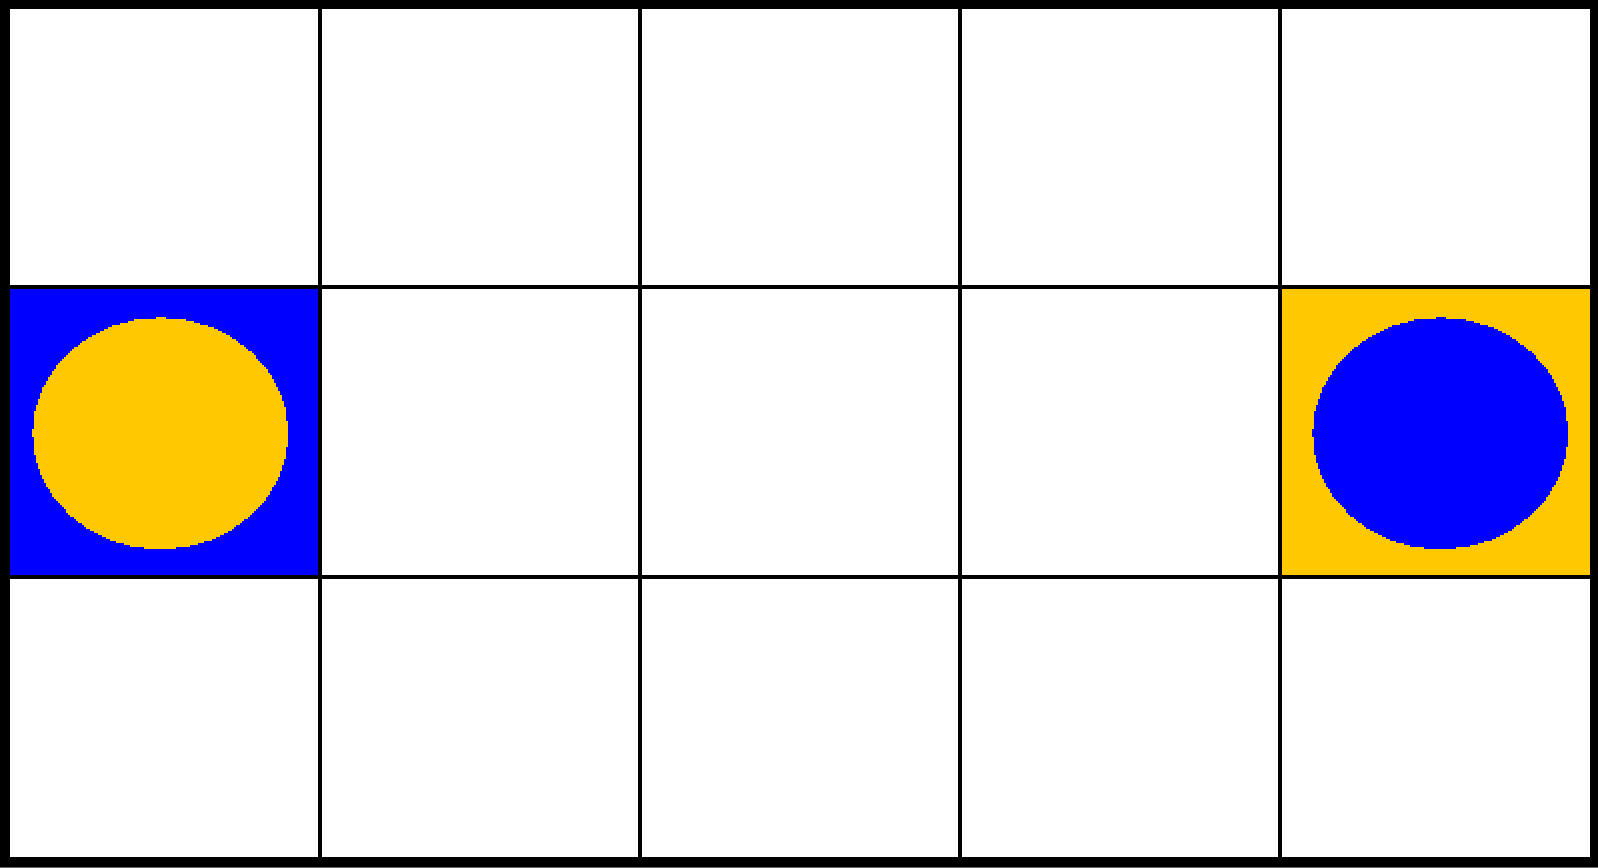
\includegraphics[width=0.65\columnwidth]{figures/threebyfive.png}
\caption{Hallway}
%\caption{Hallway, a three-by-five grid that requires a coordination strategy to efficiently play the game. Several strategies also allow an agent to defend against an uncooperative partner.}
\label{fig:hallway}
\end{subfigure}
\begin{subfigure}{.3\textwidth}
\centering
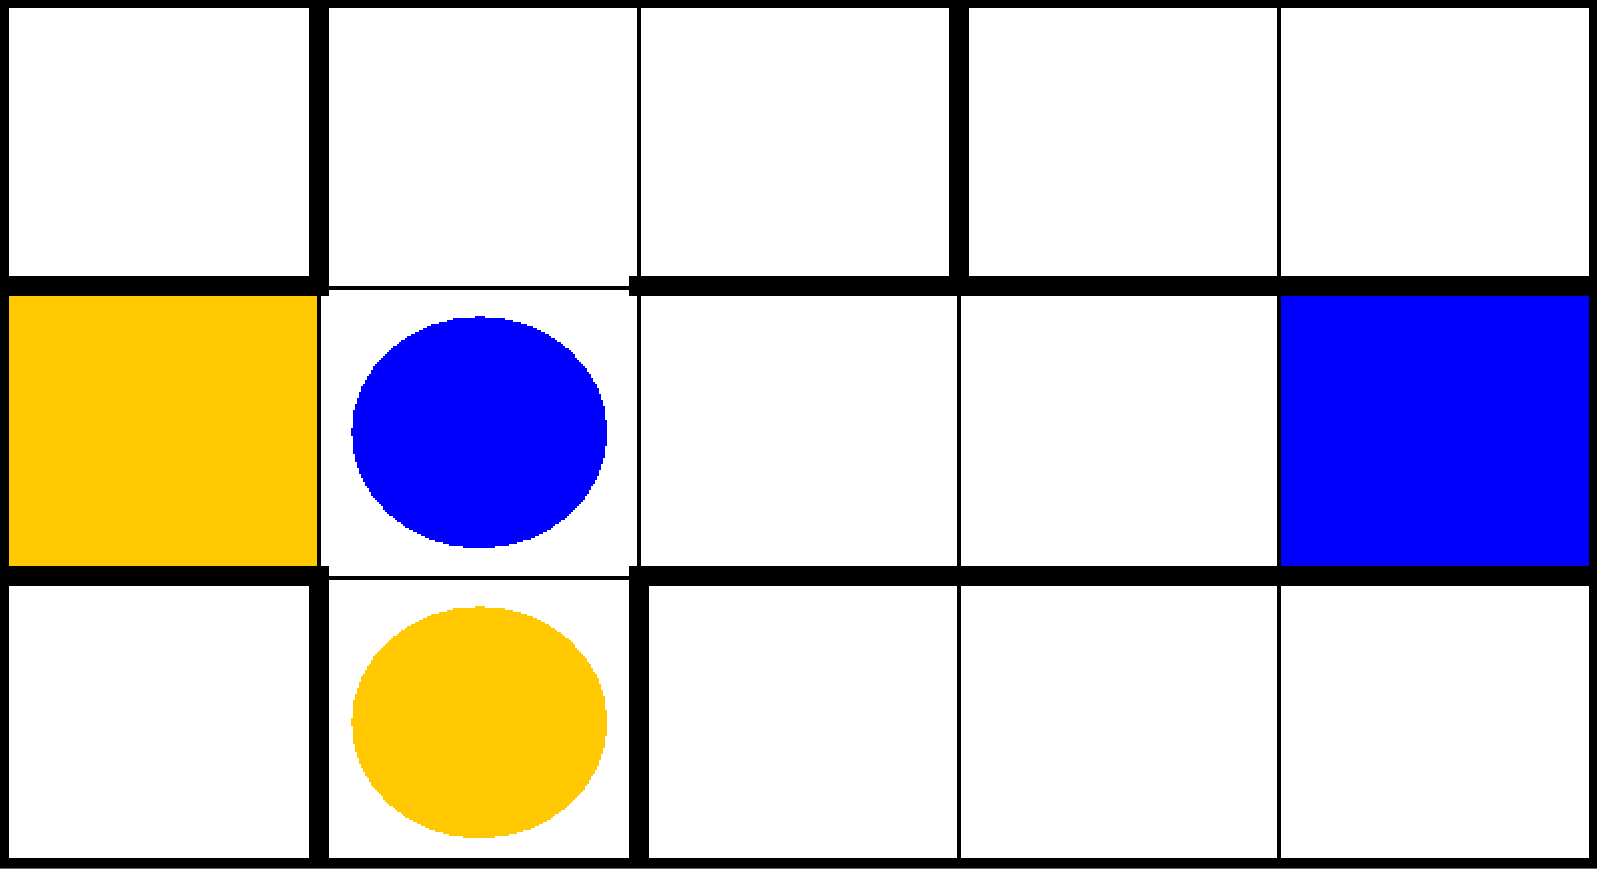
\includegraphics[width=0.65\columnwidth]{figures/threebyfivehallways.png}
%\caption{Intersection, a three-by-five grid that requires Blue to defend Orange's goal to encourage Orange to cooperate and move to the end of the uppermost hallway.}
\caption{Intersection}
\label{fig:intersection}
\end{subfigure}
\begin{subfigure}{.3\textwidth}
\centering
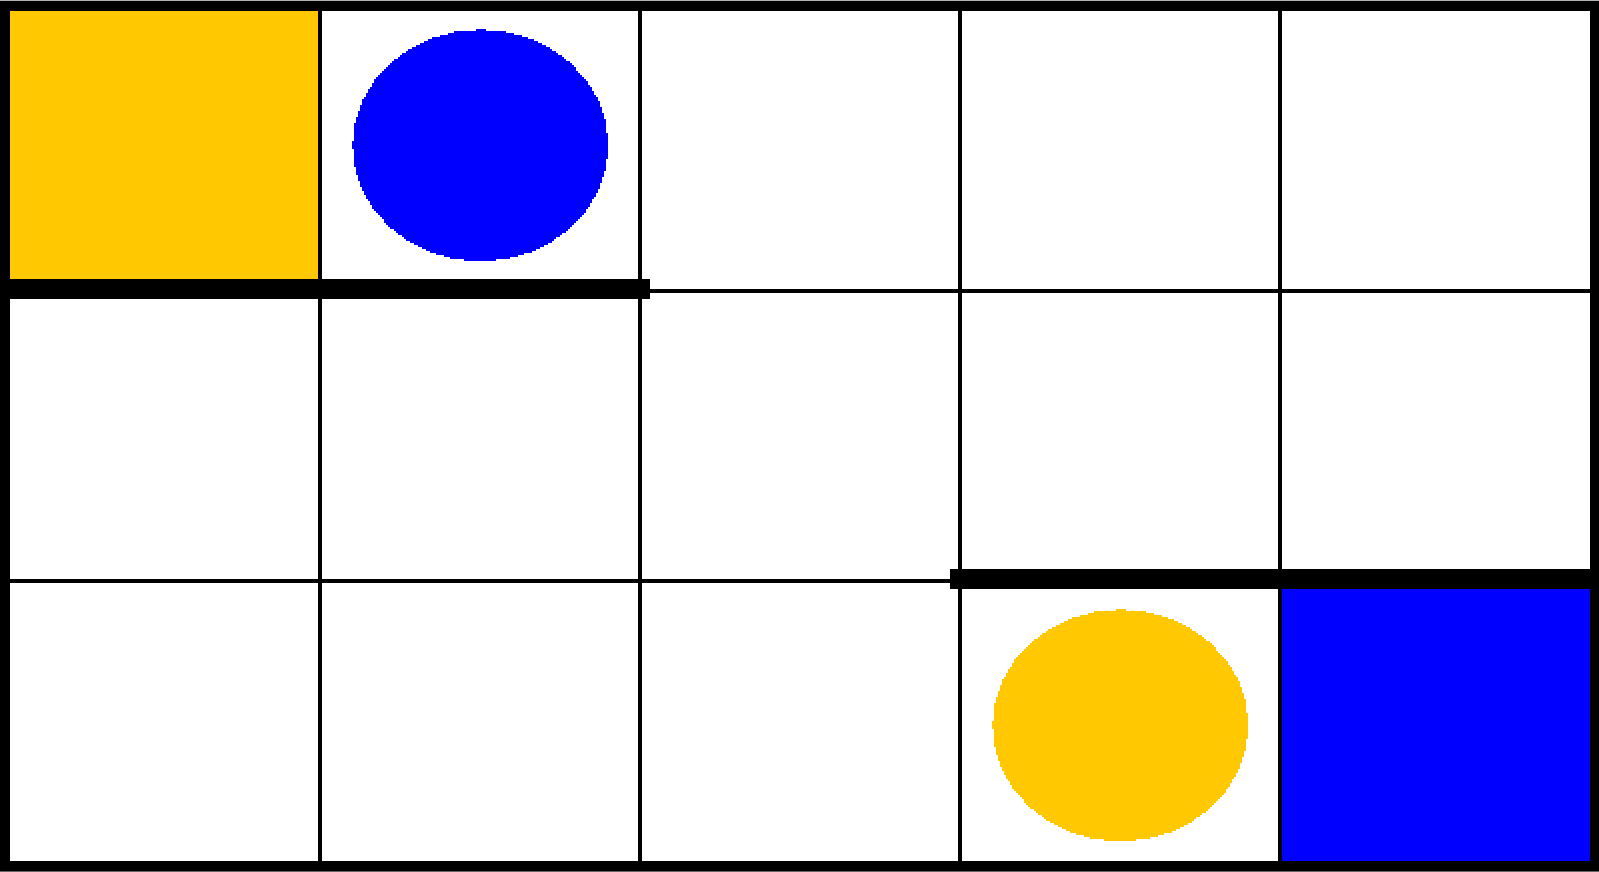
\includegraphics[width=0.65\columnwidth]{figures/threebyfivewindow.png}
%\caption{Door, a three-by-five grid that requires the partners to agree on an order in which to navigate through the center cell.}
\caption{Door}
\label{fig:door}
\end{subfigure} \\ [2.5ex]
\begin{subfigure}{.367\textwidth}
\centering

\includegraphics[width=0.5\columnwidth]{figures/longhallway.png}
\caption{Long Hall}
%\caption{Long Hall, a one-by-seven grid that allows Orange to squat on Blue's goal should they choose to not cooperate.}
\label{fig:longhallway}
\end{subfigure}
\begin{subfigure}{.367\textwidth}
\centering
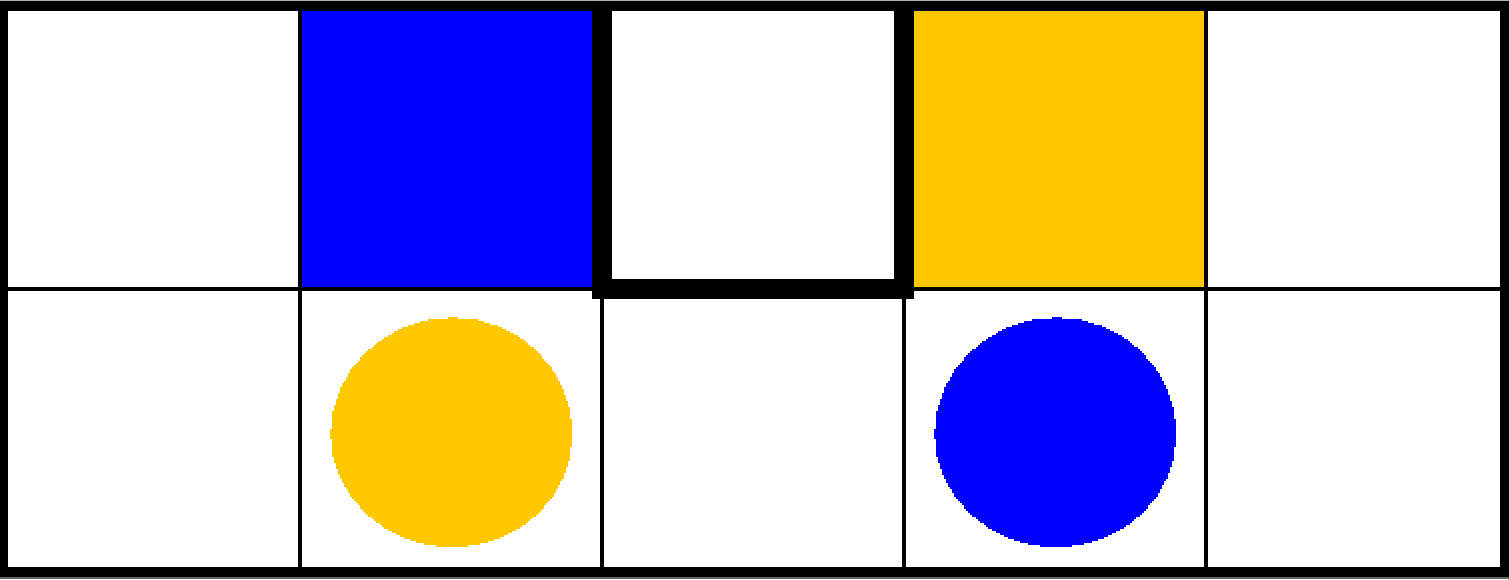
\includegraphics[width=0.5\columnwidth]{figures/nocompromise.png}
\caption{No Compromise}
%\caption{No Compromise, a two-by-five grid that requires one agent to sit on the other's goal and allow the other agent to pass, before it can move to its own goal.}
\label{fig:nocompromise}
\end{subfigure}
\caption{Five example grid games.}
\end{figure}

The grid in Figure~\ref{fig:intersection} (Intersection) requires Blue
to defend against the possibility of Orange behaving uncooperatively,
which it can achieve by squatting on the orange goal.  Orange can then
move to $(3,1)$ where both agents are equidistant from their goals.
Therefore, this game also has an equilibrium comprised of CD strategies
for both players.  

This equilibrium is not the shortest path, however.
%
Purely cooperative agents in this game could adopt a joint strategy in
which Blue moves east, while Orange waits a single step, before both
agents proceed into their goals.  This strategy profile is not
defensive for Blue though, because it does not have the opportunity to
observe if Orange will cooperate (wait) or defect (go north), and
therefore cannot defend itself if Orange decides to head straight
toward its goal.

%However, it is CD as both players are able to reach a position in
%which they are three turns from their goal without ever letting the
%other agent get closer than it is.

Figure~\ref{fig:door} (Door) is a grid that requires coordination to
navigate through the narrow center space at $(3,2)$. Any
equilibrium comprised of CD strategies for this grid must be asymmetric,
because it requires one agent to cede to the other agent the center
cell. For example, if Orange chooses to cede that cell, it should step
west into $(2,3)$ while Blue steps south into $(3,2)$. Then, Orange
needs to step east back into $(3,3)$ to prevent Blue from marching
straight into its goal. Only when Blue agrees to step aside to $(2,2)$
will they both be equidistant from their respective goals and in
position to cooperate.
%
This intricate pattern of first giving way to the opponent, and then
forcing them to step around later represents an equilibrium comprised
of CD strategies, since both agents are able to prohibit their
opponent from reaching the goal first, but still leaves open the
possibility for them both to reach their goals, cooperatively.

In the grid in Figure~\ref{fig:longhallway} (Long hall), Blue begins
one step closer to its goal than Orange does.  However, Orange can
squat on the blue goal until Blue chooses to cooperate by taking one
step back. If Orange can predict when Blue steps back, then Orange can
take one step closer to its goal while Blue steps further away, in
which case only Orange would reach its goal.  The strategy that
minimizes the risk to either agent requires that Blue wait one turn
initially, while Orange moves toward its goal.  These two strategies
comprise a CD equilibrium.

Our last grid, shown in Figure~\ref{fig:nocompromise} (No compromise),
requires not only cooperation, but both agents must also exhibit trust
for one another, or both agents cannot arrive at their goals at the
same time.  For example, Orange may sit on Blue's goal so that Blue
can move to $(1,2)$.  Then, Blue must wait two turns before both
agents are equidistant from the goals.  If Blue defects and moves
south into $(1,1)$ while Orange moves south into $(2,2)$, Orange still
has the opportunity to go back up north to block Blue from reaching
its goal.  However, if Blue moves south into $(1,1)$ when Orange steps
east into $(3,2)$, Blue will arrive at its goal sooner.  Therefore, a
trust spanning multiple rounds is required for the agents to
effectively cooperate in this game.

No equilibrium in CD strategies exists for No Compromise.  The game
is like Door in that only one player can go move through the middle
cell at a time.  Unlike Door, however, it is not possible for the
agents to simultaneously maintain a defensive position and to signal
cooperation, because any cooperative move leads to an asymmetric
situation in which the agents are no longer equidistant from their
goals.
%In other words, there's no way for one agent to signal cooperation by yielding the middle cell to the other, and then for the other agent to acknowledge that signal by moving to a position as far away from its goal as the first agent.
As a result, after one agent cooperates, there is always an incentive
for the other agent to defect, and there is nothing the cooperative
agent can do to defend itself.  Note however, that if Orange sits on
the blue goal while Blue walks to $(1,1)$ and then Blue cooperates by
waiting for Orange to walk to $(1,3)$, Blue's policy is CD.  Still,
Orange cannot respond in kind with a CD strategy; the aforementioned
strategy is C.

Taking these five grid games as an initial testbed, we performed two
pilot studies: the first involved simulations of artificial agents
playing against one another; the second pitted humans against other
humans on Mechanical Turk.  We report on the results of these
preliminary studies in the next two sections.  
%
%The main takeaway message of these experiments is that the behavior of
%both machines and humans can be at least partially explained as
%goal-driven.  In machines, those goals can be programmed directly via
%utility functions.  In humans, goals can be suggested, but the exact
%parameters governing a person's utility function are more difficult to
%control.  
%
The ultimate goal of this project, of course, is to design
artificial agents that play well with humans.  We propose to achieve
this goal by building agents that infer peoples' utility functions,
and then learn to collaborate appropriately based on these inferences.



% 1.5 pages
\begin{figure}
\centering
\begin{minipage}{0.3\textwidth}
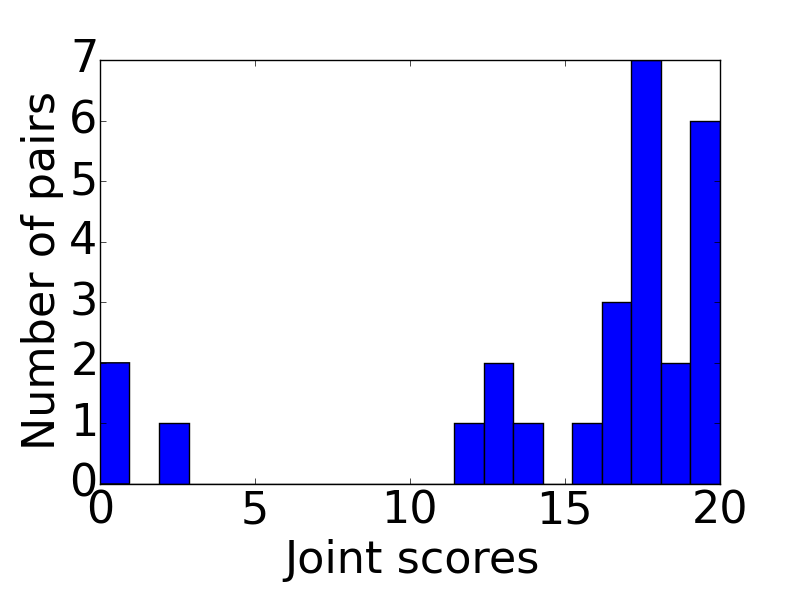
\includegraphics[width=1\columnwidth]{figures/joint_scores_team.png}
\captionof{figure}{Histograms of joint scores achieved by pairs with team treatment}
\label{fig:joint_scores_coordinated}
\end{minipage}%
\hspace{0.04\textwidth}
\begin{minipage}{0.3\textwidth}
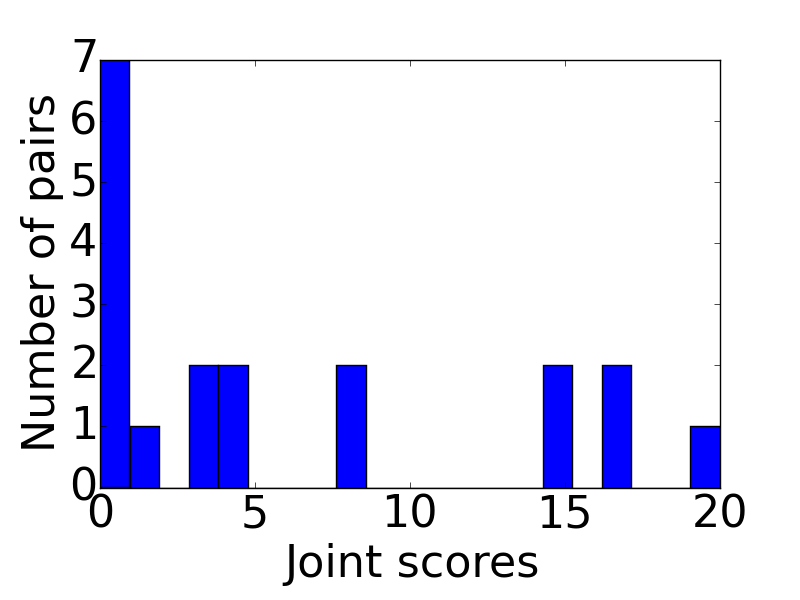
\includegraphics[width=1\columnwidth]{figures/joint_scores_individual.png}
\captionof{figure}{Histograms of joint scores achieved by pairs with individual treatment}
\label{fig:joint_scores_uncoordinated}
\end{minipage}%
\hspace{0.04\textwidth}
\begin{minipage}{0.3\textwidth}
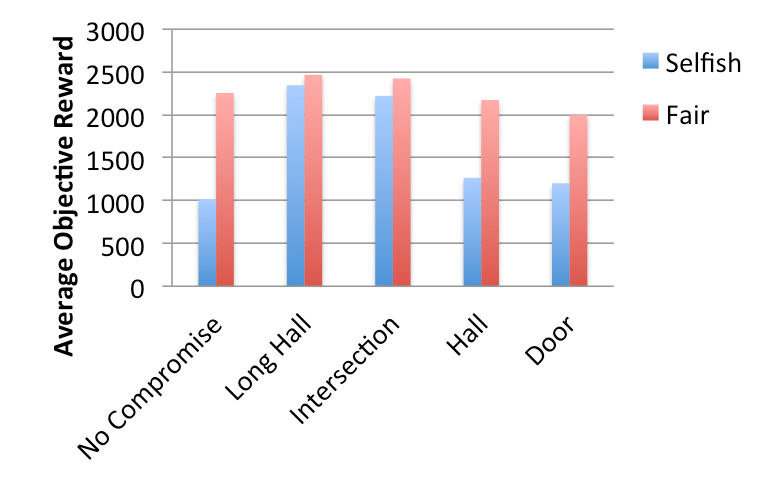
\includegraphics[width=1\columnwidth]{figures/SelfPlay.png}
\captionof{figure}{Average score of \Q-learners in self play (30,000 rounds)}
\label{f:selfplay}
\end{minipage}
\end{figure}


%\vspace{\up}
\paragraph{Simulation Experiments}
\label{sec:qlearning}

We carried out a set of simulation experiments with \Q-learning in
the grid games presented.
%
For each grid game, we conducted 50 independent runs in which two
\Q-learners faced off.  
%Runs lasted for 30,000 rounds each.  
The agents' value functions were optimistically initialized with a
value of 40 for all states and they used Boltzmann exploration with a
temperature of $0.5$.  The discount factor was set to $0.9$, and the
learning rate to $0.01$.  To ensure that the state space was
adequately explored, any state that is reachable from the initial
state had some probability of being selected as the starting position
for a round.  Once either agent reached its goal (or 100 moves were
taken), the round was terminated.  There were no step costs beyond discounting, and
rewards were 50 for reaching a goal.

We denote the outcome of a round using a pair of letters, where {\bf G} 
means the agent reached the goal and {\bf N} means the agent did not
reach the goal. The first letter in the pair represents the agent's
own outcome and the second represents its opponent's outcome. For
example, {\bf GN} is used to denote that the agent reaches its goal
while its opponent does not.

As two \Q-learning algorithms are not guaranteed to converge in
self-play, we arbitrarily stopped the learning after 30,000 rounds,
and checked the strategies learned.  In spite of \Q-learning not
explicitly seeking outcomes with high social welfare, it very reliably
identified cooperative strategies leading to {\bf GG} outcomes.
% zzz do we provide results to reference?

Only the No Compromise game posed a challenge to the \Q-learners.
There, they tend to thrash about, finding a pair of strategies that
work well together only to eventually discover that one of the agents
has an opportunity to defect.  The defection is destabilizing, so a
new search begins for strategies that work well together.  This result
is not altogether unsurprising, because No Compromise is the only game
in our testbed that does not possess a pair of CD strategies that
constitute a Nash equilibrium.

%Sometimes, \Q-learning finds strategies that are cooperative and stable,
%but these strategies are brittle and would not be successful against
%agents with other strategies.



In a second set of \Q-learning experiments, we examined the impact of
endowing agents with \mydef{social preferences}. That is, their
rewards no longer depend solely on their own successes and
failures---they depend on those of other agents in the environment as
well.

To make this idea more precise, we separate \mydef{objective} and
\mydef{subjective} reward. Objective reward is the usual reward
signal provided to the agent from the environment, and by which
behavior is judged. Standard reinforcement-learning agents, such as a
\Q-learning agent, seek to optimize their own objective reward
signal---we call this preference the ``selfish'' preference because
these agents are only concerned with their own outcomes.

In some environments, however, it useful to distinguish this objective
reward from subjective reward---the quantity the agent \emph{believes}
it should be optimizing. Previous work has shown that optimizing
subjective reward can sometimes lead agents to be more effective in
their acquisition of objective reward~\cite{singh2009rewards}.  (Indeed, we
reach this same conclusion in our experiments.)

Considering the four different outcomes in these games---{\bf GG},
{\bf GN}, {\bf NG}, {\bf NN}---there are 75 different possible
preference orderings (allowing for ties). The selfish ordering that
ignores the opponent's outcome is one of these:
{\bf GG} $\sim$ {\bf GN} $\succ$ {\bf NG} $\sim$ {\bf NN}.
%Regardless of the opponent's outcome, a selfish agent only prefers that it gets to its goal. 
Nine of the 75 orderings are consistent with the selfish ordering,
strictly preferring {\bf Gx} to {\bf Nx} for all {\bf x}.

Of particular interest is the \mydef{fair} preference, which we define
as the objective reward of the agent minus 25\% of the difference
between its own and the opponent's objective rewards:
$r_{s} = r_{a} - 0.25 \left| r_{a} - r_{o} \right|,$ where $r_{s}$
is the agent's subjective reward, $r_{a}$ is the agent's objective
reward, and $r_{o}$ is the opponent's objective reward.\footnote{Other
percentages would achieve the same result.}  By incorporating this
fairness term into the agent's subjective reward, it strictly prefers
the following ordering:
{\bf GG} $\succ$ \mbox{\bf GN} $\succ$ \mbox {\bf NN} $\succ$ {\bf NG}.
That is, the agent prefers making it to its goal as opposed to not,
but it additionally prefers that the opponent only get to its goal if
the agent itself does as well. To say it another way, a fair agent
wants its opponent to win with it or lose with it.

%%JLA: I was tempted to write here that Tit-for-Tat has a flavor of ``fairness'' preference, but I'm too tired to think through this properly.

%\begin{wrapfigure}{l}{0.4\textwidth}

%\end{wrapfigure}

Figure~\ref{f:selfplay} shows the result of the selfish and fair
agents playing against others of the same type in each of our test
grid games.  Of the nine orderings, only three (all variations of the
fair preference ordering) achieve consistent cooperation in self play
across all five grid games.  Consequently, fair agents obtain higher
total (objective) rewards than others.  
%
We also ran all nine preference orderings against one another.  The
average scores (across both players) in games involving a fair agent
tend to be higher than the average scores in games not involving a
fair agent.

\comment{
\begin{figure*}
\centering
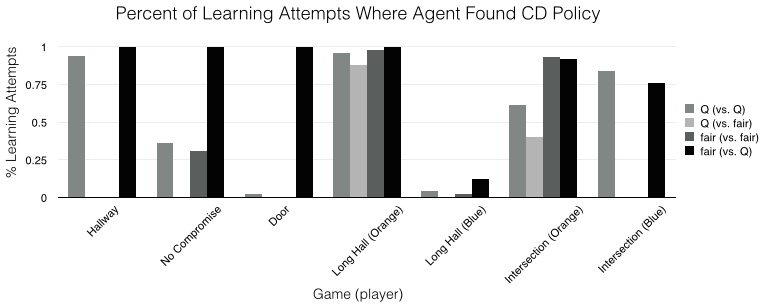
\includegraphics[width=1.5\columnwidth]{figures/ConvCD.png}
\caption{The percentage of learning attempts where the agent's final policy was CD by game and learning opponent.}
\label{f:convCD}
\end{figure*}

In Figure~\ref{f:convCD}, we show results on the classification of
policies found by the agents when learning against opponents of
different preference types. These results show that the fair agent
(\Q-learning with preferences in Equation~\ref{e:fair}) finds a CD
policy as frequently as or more frequently than normal
selfish \Q-learning when trained against another \Q-learning agent or
when trained against a fair agent. The exception is Blue in
Intersection. Across all five games and all agent positions, the
selfish agent finds a CD policy in 50.9\% attempts when learning
against selfish and in 12.8\% of attempts against the fair agent. The
fair agent's performance in these cases is 88\% and 25.5\%,
respectively. These results suggest that \Q-learners with fair
preferences may find CD policies more often, especially when they
learn against a selfish player. Whether this is general for a broader
set of grids is an important question for future work.
}

We also analyzed the types of strategies learned by fair and
selfish \Q-learners after multiple simulations of various
configurations. Interestingly, we found that \Q-learners with fair
preferences tend to find CD strategies more often, especially when
paired with selfish agents.

In summary, \Q-learners naturally learn to cooperate in the grid games
studied, discovering equilibria comprised of CD strategies when they
exist.  Cooperation can be induced in other games by manipulating
the \Q-learners' subjective rewards to incorporate the success of others.

In the next section, we describe analogous experiments conducted with
humans playing grid games.  In those experiments as well, we were able
to manipulate the rewards to favor fairness, and doing so induced more
cooperation than otherwise.

\comment{
Given the option of who to play with, agents do best when playing
against the fair preference ordering. We also analyzed which
preference ordering is the preferred one to adopt. It turns out that
the preference ordering {\bf GN} $\succ$ {\bf GG} $\succ$ {\bf NG}
$\sim$ {\bf NN} is an evolutionary stable strategy---it outperforms
competitors in a population and can maintain its dominance against
invaders. It adopts a much more aggressive stance that the fair
preference ordering in that it prefers winning alone to sharing the
top spot. Thus, it has a tendency to find strategies that drives its
opponents' scores down.
}



% 1.5 pages

%\vspace{\up}
\paragraph{Turk Experiments}
\label{sec:human}

We ran two studies in which human subjects played grid games.  We
recruited participants on Mechanical Turk to play the Hallway
game 
%(Figure~\ref{fig:hallway}) 
against another Turker.  

Each participant began with an instruction phase that used a series of
practice grids to teach them the rules of the game: arrow keys to move
north, south, east, or west in the grid; spacebar to wait; both agents
move simultaneously; when two agents try to enter the same square,
their moves fail; and the round ends when either agent reaches a goal.
Example grids demonstrated outcomes in which both agents reached a
goal, and outcomes in which one did and the other did not.  All
transitions (including transitions that did not involve changing
location) were animated so that participants could see that their
actions registered.

%An example of the instruction phase can be viewed at \url{http://goo.gl/SWme3n}. 

After the instruction phase, the participants were paired up.  Each
pair played a match consisting of 20 rounds, which ended when either
or both agents reached a goal, or when they had taken 30 actions
without either reaching a goal.

We designed two different treatments, one (the ``individual''
treatment) was a control, and the other (the ``team'' treatment) was
intended to inspire team reasoning.  In the individual treatment, a
participant received a bonus when they reached their goal, regardless
of whether the other participant also reached their goal.  In the team
treatment, a participant received a bonus only if they reached
their goal at the same time as the other member of their pair.

We recruited 40 participants to form 20 pairs in the individual
treatment; in the team treatment, we recruited 50 participants.  All
participants received \$2.00 as a base payment, and \$0.10 bonuses for
goals scored according to the rules of the treatment.



Figure~\ref{fig:joint_scores_coordinated} and 
figure~\ref{fig:joint_scores_uncoordinated} are two histograms illustrating the
distribution of joint scores achieved by the pairs in the two
treatments.  The team treatment, which in the Hallway game requires
team reasoning (because the players only succeed when they
simultaneously reach their goals), produced significantly more
successful teams.
%($p < 0.05$).\commenta{what was tested here?}
%
In particular, 19 teams (76\%) achieved a score at or above 15 points
in the team treatment, but only 3 achieved a similar score in the
individual treatment.

\begin{wraptable}{r}{0.5\textwidth}
%\begin{table}
\begin{center}
\small{
\begin{tabular}{|c|c|c|}									   
\hline
			& Individual Reasoning              & Team Reasoning 	\\ \hline
 Compete		& 32\% 					& 0\% 			\\ \hline
 Trust		& 21\% 					& 76\% 			\\ \hline
 Surrender	& 21\% 					& 8\% 			\\ \hline
 CD			& 11\% 					& 16\% 			\\ \hline
 Alternate		& 11\% 					& 0\% 			\\ \hline
 Stalemate	& 5\% 					& 0\% 			\\ \hline
\end{tabular}}
\caption{A comparison between the strategies learned by pairs in the two treatments. 
These percentages represent $19$ games in the individual reasoning experiment,
and $25$ games in the team reasoning experiment.}
\label{tab:class}
\end{center}
%\end{table}
\end{wraptable}

Table~\ref{tab:class} compares the outcomes of matches in the two
different treatments under an intuitive classification scheme, which
we based on the behavior of the participants in the final two rounds
after 18 prior rounds of learning.  We are planning much more
extensive experimentation with human participants on grid games, after
which we hope to interpret some of these classifications
(e.g., trust, CD, etc.) as types of norms.

\emph{Compete\/} means, in the final round, only one player reaches
their goal, and in the last two rounds, the players collide at least
once.  \emph{Trust\/} means both players score in the last round, but
only when one player did not take advantage of an opportunity to
defect.  \emph{Surrender\/} means that in the final two rounds, only
one player reaches the goal and does so without any collisions.
\emph{CD} (\emph{Cooperatively Defend}) means that both players score
in the final round, but each does so in a way that prevents the other
player from reaching the goal alone.  In \emph{Alternate} matches,
both players reach their goal alone exactly once in the last two
rounds, without any collisions.  Finally, in \emph{Stalemate} matches,
neither player reaches their goal in the final round.

The treatment impacts the types of behavior we observe.
The incidence of competitive behavior drops dramatically, while trust
increases threefold.  Since trust increases, surrendering becomes less
necessary, and consequently much rarer.  Also of interest, the
incidence of CD behavior doubles.  
%Perhaps people who would have engaged in competitive behavior in the individual treatment are willing to play a CD strategy in the team setting.  
%Edited 88 to 92% to correct error from chart.
Overall, 92\% of participants exhibit cooperative behavior (either
trust or CD) in the team treatment, compared to only 33\% in the
individual treatment.

%Stalemate, which  occurred only rarely even in the individual treatment, is eliminated in the team treatment.

%Table~\ref{tab:class} suggests that the team reasoning experiment encourages participants to cooperate in such a way that we can try to understand how participates find cooperative strategies given that cooperation is a shared intention,  as opposed to potentially just a personal intention.

\comment{
Figure~\ref{fig:scores_coordinated} and figure~\ref{fig:scores_uncoordinated} show plots of improving success of the matches with team-reasoning and individual reasoning respectively. Each figure contains three plots, showing results for all agents, agents which received a joint score of 10 and above and 15 and above. Each plot contains three lines showing the fraction each round ended in success, failure or a round timeout. 

All plots show an increasing measure of successful coordinations as rounds progress through each match. The plots show that the teams explicitly tasked with cooperation performed significantly better. Also, teams that scored a higher joint score converged toward optimal cooperation sooner than teams that scored lower. Teams that scored 15 points or above reached near-optimal cooperation by round 4 with both team reasoning and without, suggesting that two cooperating players needed to agree early on to achieve the best collaboration.


\begin{figure}
\centering
\begin{subfigure}{.5\textwidth}
\centering
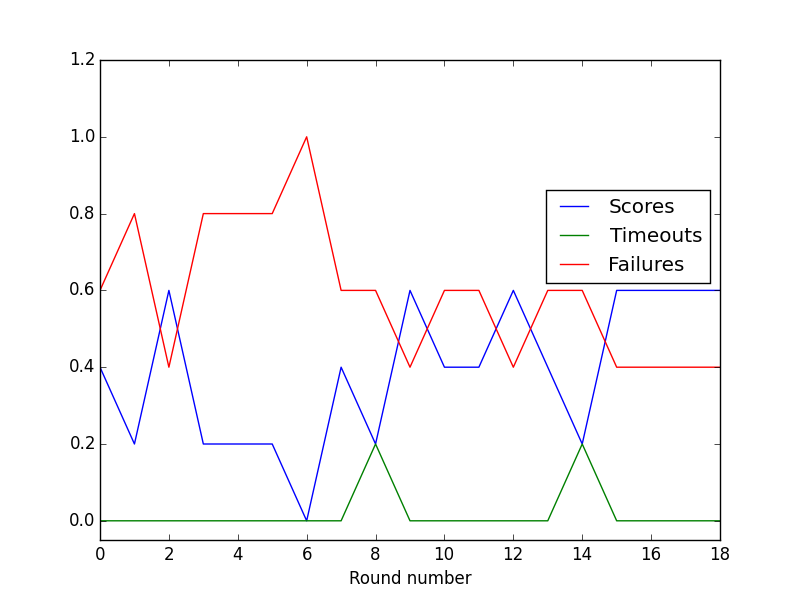
\includegraphics[width=\columnwidth]{figures/scores_coordinated_rest.png}
\caption{$< 15$ (6 teams)}
\label{fig:scores_coordinated_rest}
\end{subfigure}%
\begin{subfigure}{.5\textwidth}
\centering
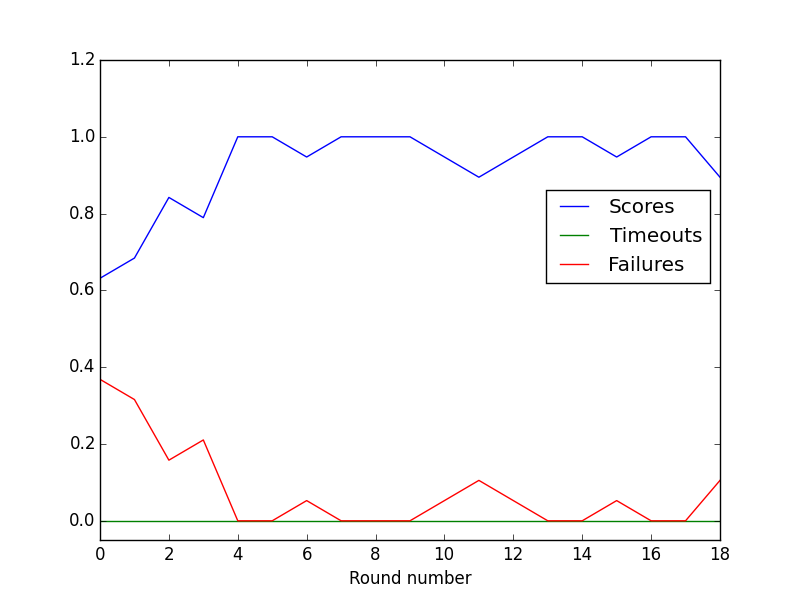
\includegraphics[width=\columnwidth]{figures/scores_coordinated_15.png}
\caption{$>= 15$ points (19 teams)}
\label{fig:scores_coordinated_15}
\end{subfigure}
\caption{Fraction of joint scores, coordination failures and round timeouts vs round number for the coordinated match group}
\label{fig:scores_coordinated}
\end{figure}

\begin{figure}
\centering
\begin{subfigure}{.5\textwidth}
\centering
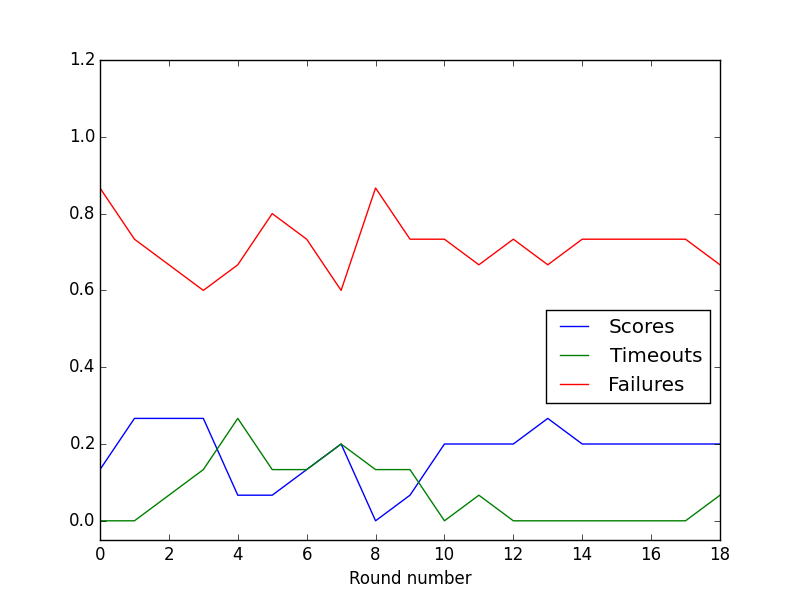
\includegraphics[width=\columnwidth]{figures/scores_uncoordinated_rest.png}
\caption{$< 15$ (17 teams)}
\label{fig:scores_uncoordinated_rest}
\end{subfigure}%
\begin{subfigure}{.5\textwidth}
\centering
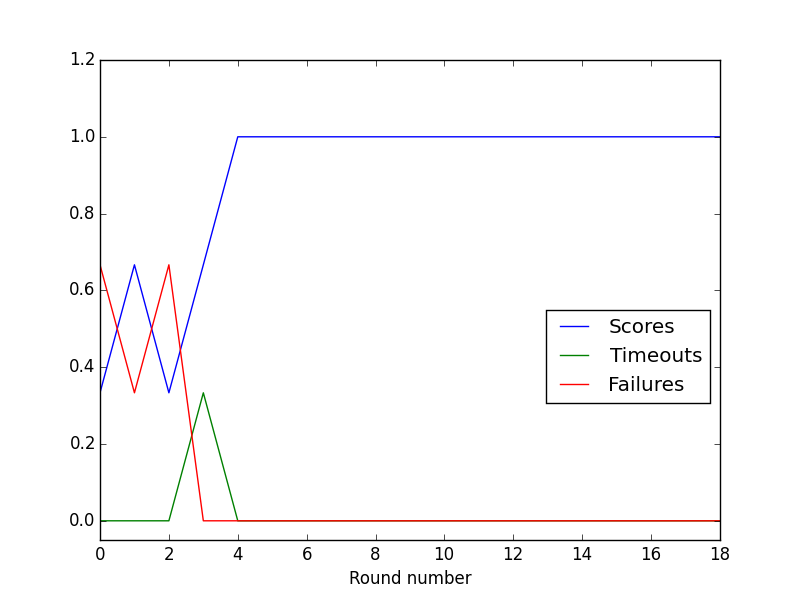
\includegraphics[width=\columnwidth]{figures/scores_uncoordinated_15.png}
\caption{$>= 15$ points (3 teams)}
\label{fig:scores_uncoordinated_15}
\end{subfigure}
\caption{Fraction of joint scores, coordination failures and round timeouts vs round number for the uncoordinated match group}
\label{fig:scores_uncoordinated}
\end{figure}


Another measure of team cooperation is the number of turns required to complete a round. Figure~\ref{fig:lengths_coordinated} and figure~\ref{fig:lengths_uncoordinated} show plots of the number of turns per round for matches with team-reasoning and with independent reasoning.

While each plot shows a lower trajectory length initially, it corresponds to lower success from figures~\ref{fig:scores_coordinated} and ~\ref{fig:scores_uncoordinated}. All matches experienced an initial increase in number of turns, but for the most cooperative teams, it quickly returns to a steady state. In the team reasoning matches, less cooperative teams experienced periodic bouts of uncoordinated rounds.

Though there were only three teams classified as cooperative in the individual reasoning group, they exhibited a more exaggerated version of the cooperative teams in the team reasoning study, suggesting that the behavior of fully cooperative teams in a more open setting will exhibit similar behaviors. For both groups of individual reasoning teams, the initial rise in the number of turns is significantly exaggerated over the team-reasoning group. 


\begin{figure}
\centering
\begin{subfigure}{.5\textwidth}
\centering
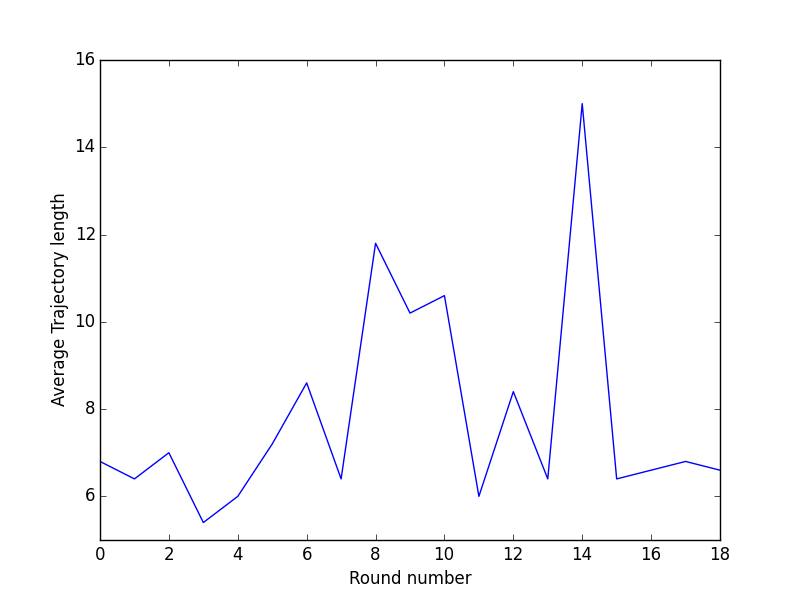
\includegraphics[width=\columnwidth]{figures/lengths_coordinated_rest.png}
\caption{$< 15$ points (6 teams)}
\label{fig:lengths_coordinated_rest}
\end{subfigure}%
\begin{subfigure}{.5\textwidth}
\centering
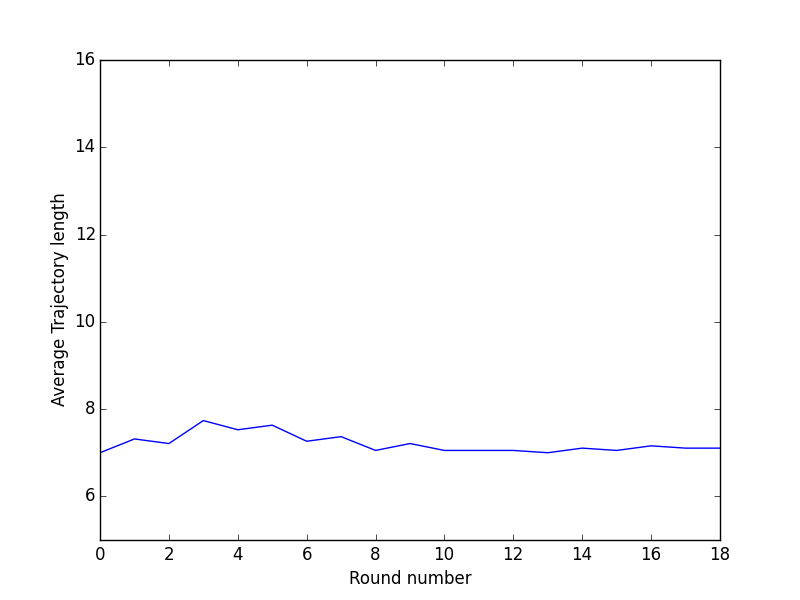
\includegraphics[width=\columnwidth]{figures/lengths_coordinated_15.png}
\caption{$>= 15$ points (19 teams)}
\label{fig:lengths_coordinated_15}
\end{subfigure}
\caption{Average number of turns per round vs round number for the team reasoning group}
\label{fig:lengths_coordinated}
\end{figure}

\begin{figure}
\centering
\begin{subfigure}{.5\textwidth}
\centering
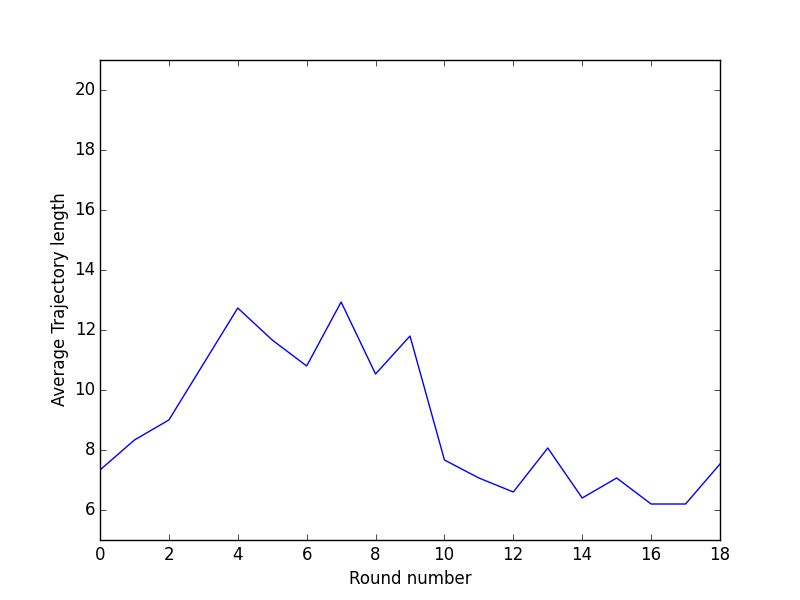
\includegraphics[width=\columnwidth]{figures/lengths_uncoordinated_rest.png}
\caption{$< 15$ points (17 teams)}
\label{fig:lengths_uncoordinated_rest}
\end{subfigure}%
\begin{subfigure}{.5\textwidth}
\centering
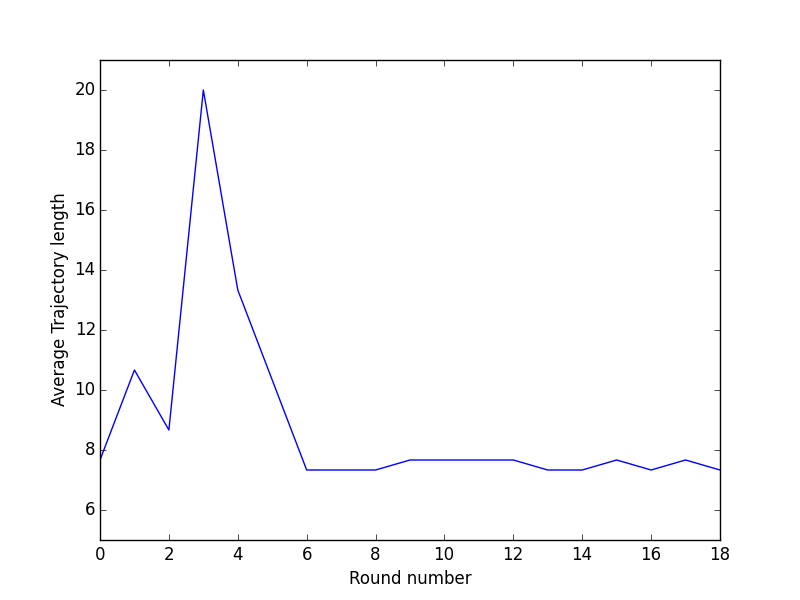
\includegraphics[width=\columnwidth]{figures/lengths_uncoordinated_15.png}
\caption{$>= 15$ points (3 teams)}
\label{fig:lengths_uncoordinated_15}
\end{subfigure}
\caption{Average number of turns per round for the individual reasoning match group}
\label{fig:lengths_uncoordinated}
\end{figure}
}

%%%subjective utility functions
The results involving human subjects playing grid games are consistent
with the results obtained in our simulations of \Q-learners playing
grid games.  In both sets of experiments, more cooperation was
achieved when the treatment incorporated social preferences.  While
the subjective utility functions of artificial agents are within our
control, so that we can perhaps lead artificial agents towards
collaborative behavior, the subjective utility functions of humans are
not.  Nonetheless, behavioral economists often infer approximations of
utility functions from experimental data by assuming some underlying
structural form, and then estimating the relevant
parameters~\cite{blanco11,fisman07}.  Likewise, one of the primary
uses of our Turk experimental framework is to generate trace data of
humans playing grid games and learning norms (such as trust, CD,
etc.), so that we can then proceed to infer utility functions and
relate them back to the norms they produce.

Next we present our proposed norm representation.  We then present an
algorithm for learning norms from trace data, human- or
machine-generated.  We also present an interactive algorithm, in which
agents can learn while at the same time establishing a norm.  We then
proceed to demonstrate the viability of our algorithms on human-human
(Turk) and agent-agent (simulation) data.  A key step in our plan for
future work is to integrate our learning algorithms with the Turk
platform, so that we can study interactive human and agent learning.

%together with an algorithm for learning norms, which, as an
%intermediate step, involves learning utility functions, which we
%ultimately do from human trace data.


% 5 pages

\section{Norm Representation}
\label{sec:representation}

Our norm representation and learning algorithms are best explained
using the formalisms of Markov decision processes and stochastic
games.  We start by providing the necessary background.
%We provide background first, and then describe our representation.

A \mydef{Markov Decision Process} (MDP) is a model of a single-agent
decision making problem, defined by the tuple $(S, A, T, R)$, where
$S$ is the set of states in the world; $A$ is the set of actions that
the agent can take; $T(s' \mid s, a)$ defines the transition dynamics:
the probability the environment transitions to state $s' \in S$
after the agent takes action $a \in A$ in state $s \in S$; and 
$R(s, a, s')$ is the reward function, which returns the reward the
agent receives when environment transitions to state $s'$ after the
agent takes action $a$ in state $s$.

The goal of planning or learning in an MDP is to find a policy $\pi :
S \rightarrow A$ (a mapping from states to actions) that maximizes the
expected future discounted reward under that policy: $E^{\pi} \left[
  \sum_{t=0}^\infty \gamma^t R(s_t, a_t, s_{t+1}) \right]$, where
$\gamma \in [0, 1]$ is a discount factor specifying how much immediate
rewards are favored over distant rewards. 
%Since this sum goes to the infinite future, this objective is called an {\em infinite horizon} objective.

To find an optimal policy, many algorithms compute the optimal state
($V^*(s)$) and state-action ($Q^*(s,a)$) value functions that specify
the expected future discount reward under the optimal policy from each
state, and from taking an action in a state and then following the
optimal policy respectively. 
%These functions are defined recursively
%by the Bellman equations:
%%
%\begin{equation}
%V^*(s) = \max_{a \in A} \sum_{s' \in S} T(s' \mid s, a) \left[ R(s, a, s') + \gamma V^*(s') \right].
%\end{equation}
%and
%\begin{equation}
%Q^*(s,a) = \sum_{s' \in S} T(s' \mid s, a) \left[ R(s, a, s') + \gamma V^*(s') \right].
%\end{equation}
%\noindent
Given these functions, the optimal policy is derived by taking an
action in each state with the maximum Q-value: 
$\pi(s) \in \arg\max_{a \in A} Q(s, a)$~\cite{bertsekas87}.

\mydef{Inverse reinforcement learning} (IRL) is a class of a {\em
  learning from demonstration} (LfD) problem. An LfD problem is a
problem in which an agent is presented demonstrations of behaviors and
must learn a policy of behavior that closely reproduces the observed
behavior. In IRL, an agent learns this policy indirectly by learning a
reward function for the MDP that describes an environment that would
motivate an agent to behave in a way that is consistent with the
observed behavior. A strength of the IRL formulation is that simple
reward functions can often capture complex behavior. As a result, a
learned reward function can often produce behavior that accurately
generalizes the observed behavior to many states, including states not
observed in the input demonstrations.

Although there are multiple IRL formalizations and approaches, they
all take as input an MDP together with a \mydef{family} of a reward
functions $R_\Theta$ that is defined by some parameter space $\Theta$,
and a dataset $D$ of trajectories (where a trajectory is a finite
sequence of state-action pairs: $\langle (s_1, a_1), ..., (s_n, a_n)
\rangle$). The algorithms then output a specific parameterized reward
function $R_\theta \in R_\Theta$, which induces a policy that is
consistent with the input trajectories.
%
Different IRL algorithms frame the objective function for policy
consistency differently. One common approach is to treat the
search problem as a probabilistic inference
problem~\cite{babes11,lopes2009active,ramachandran2007bayesian,ziebart2008maximum}. 

\comment{
For example, in the maximum-likelihood setting~\cite{babes11}, the
goal is to find a reward function parameterization that maximizes a
likelihood function:
%
\begin{equation}
\label{eq:mlirl}
\theta \in \arg\max_{\theta} L(D \mid R_{\theta}) = \prod_{t \in D} \prod_i^{|t|} \pi_{\theta}(s_i, a_i),
\end{equation}

where $\pi_{\theta}(s, a)$ is a stochastic policy defining the
probability of taking action $a$ in state $s$ when the parameterized
reward function to be maximized is $R_{\theta}$. Typically, the
Boltzmann (softmax) stochastic policy over the $Q$-values is used:
$\pi_{\theta}(s, a) = \frac{e^{\beta Q_{\theta}(s,a)}}{\sum_{a' \in A}
  e^{\beta Q_{\theta}(s,a')}}$, where $Q_\theta(s, a)$ is the $Q$-function
when the reward function is parameterized by $\theta$.
}

The stochastic games formalism can be viewed as an extension of MDPs
to the multi-agent case~\cite{littman1994markov}. 
%In a stochastic game, each of the agents in the environment make decisions simultaneously at each discrete time step and can only observe the other agents' decisions after all decisions have been made and executed in the environment. 
A \mydef{stochastic game} is defined by the tuple $(I, S, A^I, T,
R^I)$, where $I$ is an index set of agents in the environment; $S$ is
the set of states of the environment; $A^I$ is set of actions for each
of the agents with $A^i$ denoting the action set for agent $i \in I$;
$T(s' \mid s, j)$ is the transition dynamics specifying the
probability of the environment transitioning to state $s' \in S$ when
the {\em joint action} $j \in \times_i A^i$ of all agents is taken in
state $s \in S$; and $R^I$ is a set of reward functions for each agent
with $R^i(s, j, s')$ denoting the the reward received by agent
$i \in I$ when the environment transitions to state $s' \in S$ after
the agents take joint action $j \in \times_i A^i$ in state $s \in S$.

The goal in a stochastic game is to find a joint strategy that
satisfies some solution concept. Different solution concepts for
stochastic games have been explored in the past including minimax,
Nash, correlated, and CoCo equilibria
\cite{GreenwaldHall:03,HuWellman03,Littman01,ZGL:06}. There are
problems with these approaches, however. First, the resulting planners
must solve for game-theoretic equilibria in an inner loop, a problem
which in the case of Nash equilibrium, for example, is notorious for
its computational intractability~\cite{daskalakis2009complexity}. Second, in the
general case of non-constant sum games, none of the planners that make
reasonable assumptions about agent behavior yield unique joint plans,
and furthermore, none has solved the ensuing equilibrium selection
problem suitably.

Immediately generalizing from the case of MDPs, the goal of inverse
reinforcement learning in stochastic games is to learn a set of reward
functions for the stochastic game that describe an environment that
would motivate the agents to behave in a way that is consistent with
the observed behavior under some solution concept such as a Nash
equilibrium~\cite{reddy2012inverse}.  This problem, however, is
exceedingly difficult, because the planning that is necessary in the
inner loop of an IRL algorithm is subject to the challenges identified
by the equilibrium planners mentioned above.

In this project, we plan to develop IRL algorithms that can explain
norm-adhering behavior in a stochastic game.  In our preliminary
studies, we assume players' rewards are known, and our goal is to
recover a \mydef{social reward function} that combines these known
rewards in such a way as to capture a social norm expressed in the
joint play of the agents (when one exists).

%This social reward function is our norm representation.

Like the players' reward functions, a social reward function operates
on states, joint actions, and next states: $R^S : S \times_i A^i
\times S$.  In our initial model, we assume that this social reward
function can be written as linear combination of a \mydef{team
  function}, which represents team goals,
%an \mydef{individual function}, which represents an individual's goals,
and a family of what we call \mydef{bias functions} ($B_\Theta$)
defined by some parameter space $\Theta$.  The team function takes as
input a multi-agent reward function ($R^I)$, and returns a single
numeric value for any state-joint action-next state triple that
represents a team goal. One example of such a function is total
welfare (i.e., the sum of all agent rewards): 
${\mathcal T}(R^I, s, j, s') = \sum_i R^i(s, j, s')$.
%
The bias function family is similar in nature to a reward function
family that would be input to a classic IRL algorithm, but operates on
state-joint action-next state triples, thereby encoding a bias that
motivates norm-adhering behavior in games.  In addition to the
parameters of the bias function, the social reward function may also
include a parameter
%$\alpha$ 
to trade-off the team rewards against the biases.
%$R^S(s, j, s') = \alpha {\mathcal T}(R^I, s, j, s') + (1-\alpha) B_\Theta(s, j, s')$.
%but in the simplest case, $\alpha = 0.5$.

\comment{
\commenta{The individual function \ldots} \jmnote{Do we want to add
  an individual function here? Right now the social reward function
  in the pseudocode (and results) do not include an individual term.
  It also makes the batch mode less straight forward because
  it means there would be a different social reward function
  for each agent. Would that mean we run batch once for each agent?
  I'm going to comment it out for now, but we can add it back.}
}

%\jmnote{Not sure this whole above paragraph that I added is needed here; maybe best to incorporate the ideas earlier, but I was trying to bridge to why we care about features}

Recall our working definition of a social norm as a behavioral
instruction that members of the community expect one another to
follow.  This definition suggests that norms could potentially be
learned in a supervised fashion simply by learning a function that
maps states to joint actions directly, rather than capturing norms in
a social reward function that motivates joint actions.
%\commenta{do you mean just hard code a norm in the bias functions? 
%does something like this next sentence capture what you mean?}
%\commenta{This definition suggests that norms could be directly encoded in the bias functions of a social reward function as bonuses associated with specific joint actions.}
However, as an environment and a target policy become more complex,
directly learning the policy becomes more challenging, and
generalizing from it likely less successful.  As with standard IRL,
the advantage of learning a social reward function instead is that
simple reward functions can often induce complex
behaviors \emph{across states}.  For example, consider a seemingly
straightforward norm that two agents approaching one another each stay
to their right.  If the action space is over low-level controls (e.g.,
rotations and small movements) and the policy is context dependent
(e.g., navigating obstacles to get to the right side), implementing
all the joint action rules necessary to make the agents pass on the
right could be difficult to specify (and hence, learn).  However, a
social reward function can simply define a bonus for when the agents
move past each other on the right and the planning algorithm does the
rest.

%\commenta{this is a seaparte point}
%trade offs between the team goal and biases for norms can be learned. 

To facilitate social reward functions that generalize, the bias
function family must operate on a set of useful features.  As part of
this project, we plan to investigate whether existing state-of-the-art
feature selection methods for
RL~\cite{diuk2009adaptive,kolter2009regularization,li2009reinforcement,parr2008analysis}
work well in our setting, and then to work towards developing new
methods to the extent necessary.

%A viable alternative might be to design the bias functions such that
%agents can receive a bonus as they move past each other on the right.
%The intent is that motivating the desired behavior in this way would
%result in greater generalization power.  To facilitate this kind of
%generalization, the bias function family must operate on a set of
%useful features.  As part of this project, we plan to investigate
%whether existing state-of-the-art feature selection methods for
%RL~\cite{diuk2009adaptive,kolter2009regularization,li2009reinforcement,parr2008analysis}
%work well in our setting, and then to work towards developing new
%methods to the extent necessary.

%\jmnote{I made a bit of a bold claim here saying that we would investigate feature selection. I say that because this might indeed be an interesting space that benefits from new kinds of features, but if we don't want to commit to this, we can just say its outside the scope of our work.}

\comment{
We believe that the choice to represent norms by a single social
reward function is grounded in sound psychology because\commenta{JOE!!??}.
%
Furthermore, this assumption is essential for our approach to be
tractable, because IRL in MDPs is becoming increasingly easier, while
IRL in stochastic games remains enormously challenging.
}



\section{Norm Learning}
\label{sec:learning}

Given our representation of norms by a social reward function that is
parameterized by a family of bias functions, our approach to learning
norms is simply to optimize those parameters to best match observed
behavior.  We consider two forms of norm learning.  The first is
\mydef{batch} learning, in which an agent learns offline from batches
of demonstrations of other agents conforming to a norm.  The second is
\mydef{interactive} learning in which an agent learns about the
behavior of a set of unknown agents, while at the same time
interacting with them and establishing norms.

%We consider learning norms under two different conditions. First, when
%an agent observes example behaviors of other agents conforming to a
%norm, and also when an agent must interact with a set of unknown
%agents and develop new norms that facilitate coordination. We refer to
%the first learning situation as {\em batch} norm learning, since the
%agent will receive batches of demonstrations and can perform norm
%learning offline from them; we refer to the latter situation as {\em
%  interactive} norm learning, since the agent must learn norms with
%other agents while interacting with them.%

%To perform both batch and interactive norm learning, we take an
%approach in which the agent reasons about the multi-agent interaction
%as a joint task to solve and then learns biases for behavior in the
%joint task that when coupled with the overall joint task goal, results
%in norm-following behavior. To formalize and solve this learning
%problem, we build from Markov decision process and stochastic games
%formalisms, and inverse reinforcement learning literature. We first
%describe relevant background material on these topics and then
%describe our norm-learning algorithms.



%\vspace{\up}
\paragraph{Batch Learning}
\label{sec:batch}

The batch learning setting is similar to the standard IRL problem in
that the algorithm is given a batch of demonstrations and a family of
reward functions over which to search. In our case, however, the batch
data consists of trajectories of states and joint actions in a
stochastic game, and the reward function family is a social reward
function family.  To learn the parameterization of the social reward
function family that best captures the behavior exhibited in the
demonstrations, we convert the stochastic game into an MDP,
%(in which joint actions correspond to actions, etc.),
and then use IRL to learn a parameterization of the reward function
family in this MDP.

\begin{algorithm}[t]
\caption{Batch\_Learning($(I,S,A^I,T,R^I), \gamma, D, {\mathcal T}, B_\Theta$)}
\label{alg:srl}
\begin{algorithmic}
\Require stochastic game $(I,S,A^I,T,R^I)$; discount factor $\gamma$; multi-agent norm-following demonstrations $D$; team function ${\mathcal T}$; and parameterized bias function family $B_\Theta$.
\State $A^M := \times_i A^I$ \Comment{Joint action set}
\State $R^M(s, a, s') := {\mathcal T}(R^I, s, a, s')$ \Comment{Team reward function}
\State $R^S_\Theta(s, a, s') := R^M(s, a, s') + B_\Theta(s, a, s')$ \Comment{Social reward function family}
\State $R^S_\theta :=$ IRL($(S,A^M,T,R^S_\Theta), \gamma, D$)
\State \Return $R^S_\theta$ \Comment{Learned social reward function}
\end{algorithmic}
\end{algorithm}

%The batch learning algorithm is shown in Algorithm~\ref{alg:srl}
Pseudocode for the batch learning algorithm is shown in Algorithm~\ref{alg:srl}.
%
The algorithm takes as input a stochastic game; a discount factor; a
set of multi-agent demonstrations (which perhaps shows adherence to
some norm); a team function; and a family of bias functions defined by
some parameter space $\Theta$. 
%
Since the demonstrations are a set of trajectories of state-joint
action pairs, specifying the behavior of all the agents in the
environment, the first step of the batch learning algorithm is to
transform the stochastic game into an MDP. For the most part, this
transformation is straightforward: the states are the same, the MDP
action set is the space of joint actions, and the MDP transition
dynamics still operate on joint actions (which is the action set in
the MDP). A family of social reward functions is then defined as a
linear combination of the input team function (which depends on the
stochastic game's reward functions), and the family of bias
functions.\footnote{A parameter controlling the linear
combination of the team and bias function may be optimized as well.}
%
After learning a social reward function, any single agent can then
behave by selecting a joint action from the policy that results from
it, and then selecting their individual action from the joint. That
is, agent $i$ takes action $j^i \in A^i$, where 
$j \in \arg \max_j Q_{R^S_\theta}(s, j)$.

%Additionally, we set the zero-horizon value of states in  RHIRL to the team value function. Setting the zero-horizon state values to the team value function allows RHIRL to use a short horizon a with bias function family that uses all of it representation power to express behavior biases rather than the ultimate task goals. To demonstrate that property, consider the fact that the RHC with a horizon of one and a bias function that always returns zero, always returns the original team value function when its horizon-zero state values are set to the team value function. The same is true for any horizon $h \ge 0$. As a result, the bias function only needs to focus its representation power on values that motivate norm-adhering behavior and the horizon used only needs to be large enough to motivate behavior that can exploit the bias values. Since computing the team value function only has to performed once and since we expect preferences for behavior to only require small horizons to exploit in practice, we expect the social reward function learning algorithm to be very computationally efficient.

Although any off-the-shelf IRL algorithm would be applicable here, in
practice we use \mydef{receding horizon IRL}
(RHIRL)~\cite{macglashan15b}. IRL algorithms are typically
computationally demanding because they require planning in their inner
loops.
%If the social reward function learning is going to be used in any
%moderately interactive setting, this limitation may be prohibitive. 
RHIRL addresses this limitation by replacing the usual
infinite-horizon policy with a receding horizon controller (RHC) that
only plans out to some finite horizon from any given state, thereby
bounding computation time. An RHC tends to steer an IRL algorithm
towards a reward function with shaping values: short-term rewards that
guide the agent in the right direction without having to plan too far
ahead. Since these are precisely the kinds of values we want our bias
functions to capture, RHIRL allows us to plan with a short horizon,
thereby saving on computation time, which enables interactive
learning, described next.


%\vspace{\up}
\paragraph{Interactive Learning}
\label{sec:interactive}

In the interactive norm-learning setting, an agent plays with a set of
unknown agents, with whom it can potentially establish new
norms. Pseudocode for our interactive norm-learning algorithm is shown
in Algorithm~\ref{alg:inl}. The algorithm takes as input the same
arguments as the batch learning algorithm, except it includes an index
specifying which agent in the stochastic game the learner is, and it
does not include the batch of demonstrations. The agent begins by
initializing its policy arbitrarily.%
\footnote{In practice, the policy can be initialized to the agent's role
in the joint policy that follows from the team function alone.}
%
The first round of interaction produces a trajectory of joint behavior
that the learner can now learn from.  It does so by running our batch
learning algorithm on the single trajectory of experience acquired
thus far.  It then proceeds to follow the learned policy in the next
round.  After the second round completes, the agent now has two
trajectories on which it can run batch learning to update its social
reward function and its behavior.  This process then repeats for all
rounds of interaction.  
%
Note that updating the policy after each round requires computing the
$Q$-values under the newly learned social reward function.  However,
in practice, this computation can be performed lazily for each state
the agent observes in the next interaction.

\begin{algorithm}[t]
\caption{Interactive\_Learning($(I,S,A^I,T,R^I), k, \gamma, {\mathcal T}, B_\Theta$)}
\label{alg:inl}
\begin{algorithmic}
\Require stochastic game $(I,S,A^I,T,R^I)$; agent index $k$; discount factor $\gamma$; team function ${\mathcal T}$; and parameterized bias function family $B_\Theta$.
\State initialize policy $\pi^k$ arbitrarily
\State $A^M := \times_i A^I$ \Comment{Joint action set}
\State $D := \{\}$
\For{each round of play}
\State play round following $\pi^k$ %while recording the trajectory $t$
\State append new trajectory of play to $D$
%$D := D \cup \{t\}$
\State $R^S_\theta :=$ Batch\_Learning($(I,S,A^I,T,R^I), \gamma, D, {\mathcal T}, B_\Theta$)
%NO SPACE!
%\State compute $Q_{R^S_\theta}$
\State $\forall s \in S$, $\pi^k(s) := a^k \in A^k$ where $a \in \arg \max_a Q_{R^S_\theta}(s, a)$
\EndFor 
\end{algorithmic}
\end{algorithm}

%Larger RHIRL horizon can allow for more temporally abstract norms to be encoded 
%ex: "pass on the left" may take multiple steps to coordinate and give a reward when agents pass each other on the left

%\vspace{\up}
\paragraph{Norm Learning Results}
\label{sec:results}

We now present preliminary results demonstrating that both our batch
and interactive norm learning algorithms can produce reasonable
results in grid games. For batch learning, we hard code examples of
agents following different norms, and show that our algorithm is able
to recover the appropriate norm when it is trained on demonstrations
of behavior following that norm. We also show that the learned norm
can generalize to sensible behavior in other situations by testing the
agents in similar grid games after learning. For interactive learning,
we show that two agents playing together can very quickly 
%(typically after one round) 
establish a norm, and that restarting learning from scratch can result
in the agents establishing different norms.

For both sets of experiments, we examine behavior in Hallway.  The
social reward function consists of a total welfare team reward
function and a linear family of bias functions. The bias functions
operate on 50 state-joint action binary features. The first 25
features are an indicator variable for selecting one of the 25 joint
actions when the agents are in {\em conflict} and the latter 25
features are indicator functions for selecting one of the 25 joint
actions for when the agents are not a conflict. We define the agents
to be in conflict when they are in the same row of the grid and each
is closer to their opponent's goal than they are to their own
goal. Additionally, when one of the agents is one step away from their
goal, none of the features activate, thereby preventing norm
preferences from favoring premature termination of the joint
task. Since these features directly encode preferences for joint
actions rather than higher-level goals, when training we use RHIRL
with a horizon of 1. We do not expect this set of features to be
complete or capable of capturing all the possible norms that might be
established in a grid game. So an important area for future work is to
identify expressive features that can also generalize
well. Nevertheless, the features used here provide a proof of concept
for our approach.
%which can later be extended to more expressive features.

%\subsection{Batch Training Results}

\begin{figure}
    \centering
    \begin{subfigure}[b]{0.275\textwidth}
        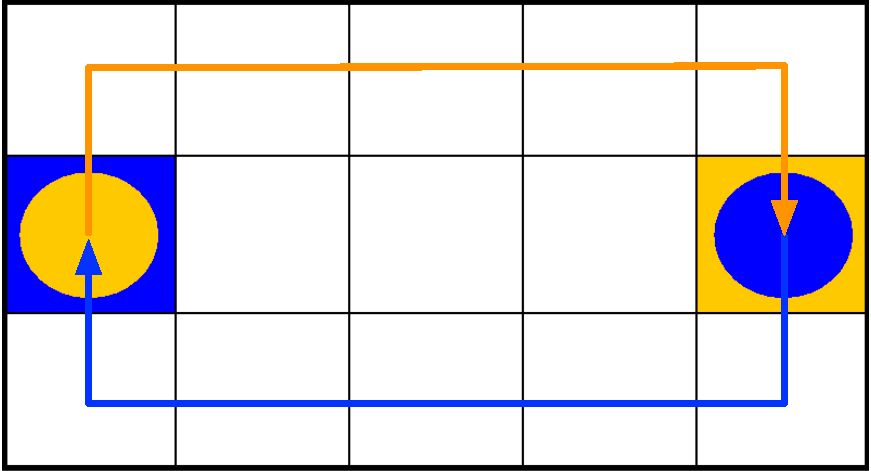
\includegraphics[width=\textwidth]{figures/batch1}
        \caption{}
        \label{fig:batch1}
    \end{subfigure}
\qquad
    ~ %add desired spacing between images, e. g. ~, \quad, \qquad, \hfill etc. 
      %(or a blank line to force the subfigure onto a new line)
    \begin{subfigure}[b]{0.275\textwidth}
        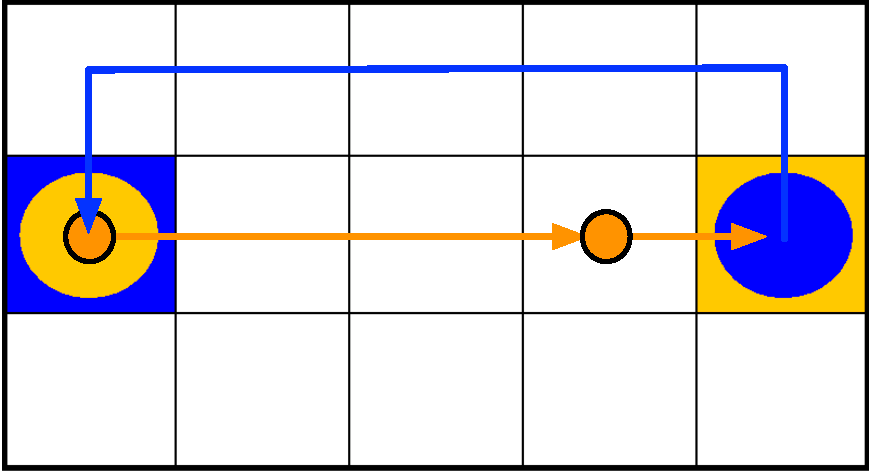
\includegraphics[width=\textwidth]{figures/batch2}
        \caption{}
        \label{fig:batch2}
    \end{subfigure}
\qquad
    ~ %add desired spacing between images, e. g. ~, \quad, \qquad, \hfill etc. 
    %(or a blank line to force the subfigure onto a new line)
    \begin{subfigure}[b]{0.275\textwidth}
        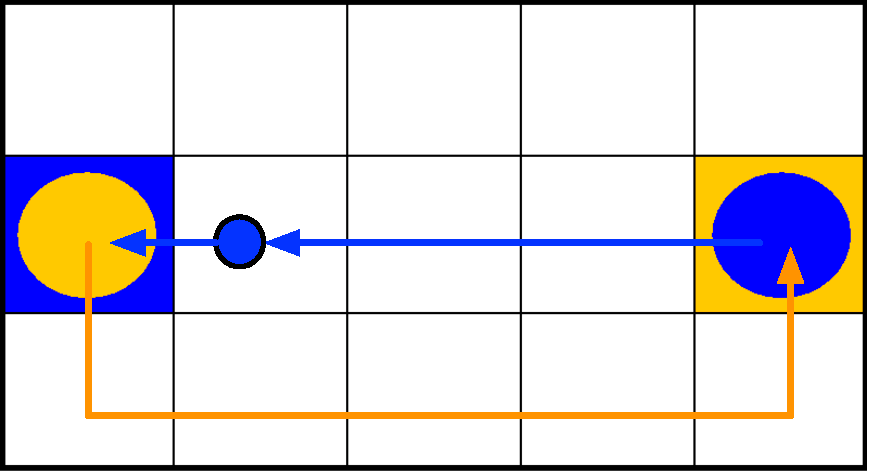
\includegraphics[width=\textwidth]{figures/batch3}
        \caption{}
        \label{fig:batch3}
    \end{subfigure}
    \caption{The three different norms the batch learning algorithm trained on in Hallway. Colored arrows indicate the path of the player of the same color. A small circle indicates a wait action.}\label{fig:batchRes}
\end{figure}

We tested our batch learning algorithm on datasets in which
agents followed three different norms. 
%All three norms are shown in \ref{fig:batchRes}. 
The first norm (Figure~\ref{fig:batch1}) shows the orange player going
north and then along the top row of the grid while the blue player
goes south and then along the bottom row. The second norm
(Figure~\ref{fig:batch2}) shows the blue player going north and along
the top row while the orange player waits, then goes east, and then
waits again for blue to catch up so they can enter their goals
together.  The third norm (Figure~\ref{fig:batch3}) has the orange
player go south and along the bottow row while the blue player
immediately goes west toward its goal and then waits two steps.
%for orange to catch up so they can enter their goals together.

For each of these three norms we generated five demonstrations, two of
which described the norm exactly, and the other three of which
contained slight deviations from the norm (for example, moving back to
the center row before reaching the end). We then
separately trained our batch algorithm on each set of demonstrations.
In all cases, the learned social reward function motivated
behavior that consistently replicated the observed norm on which it
was trained. Additionally, we planned using the learned social reward
function in a larger 7x3 hallway grid game, and obtained the same norm
behavior.

%\subsection{Interactive Training}
%\jmnote{I will also try to run an experiment in which one player is initially biased to show that the other agent adapts to them.}

\begin{figure}
    \centering
    \begin{subfigure}[b]{0.18\textwidth}
        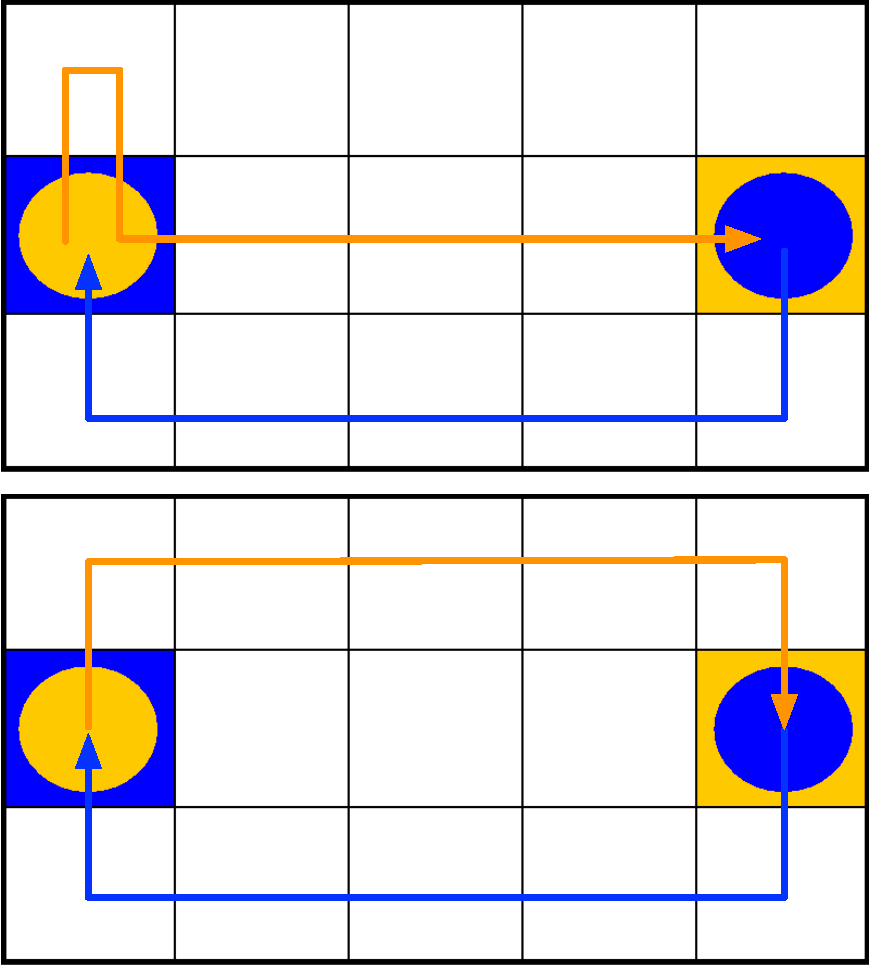
\includegraphics[width=\textwidth]{figures/interactive1}
        \caption{}
        \label{fig:inter1}
    \end{subfigure}
    ~ %add desired spacing between images, e. g. ~, \quad, \qquad, \hfill etc. 
      %(or a blank line to force the subfigure onto a new line)
    \begin{subfigure}[b]{0.18\textwidth}
        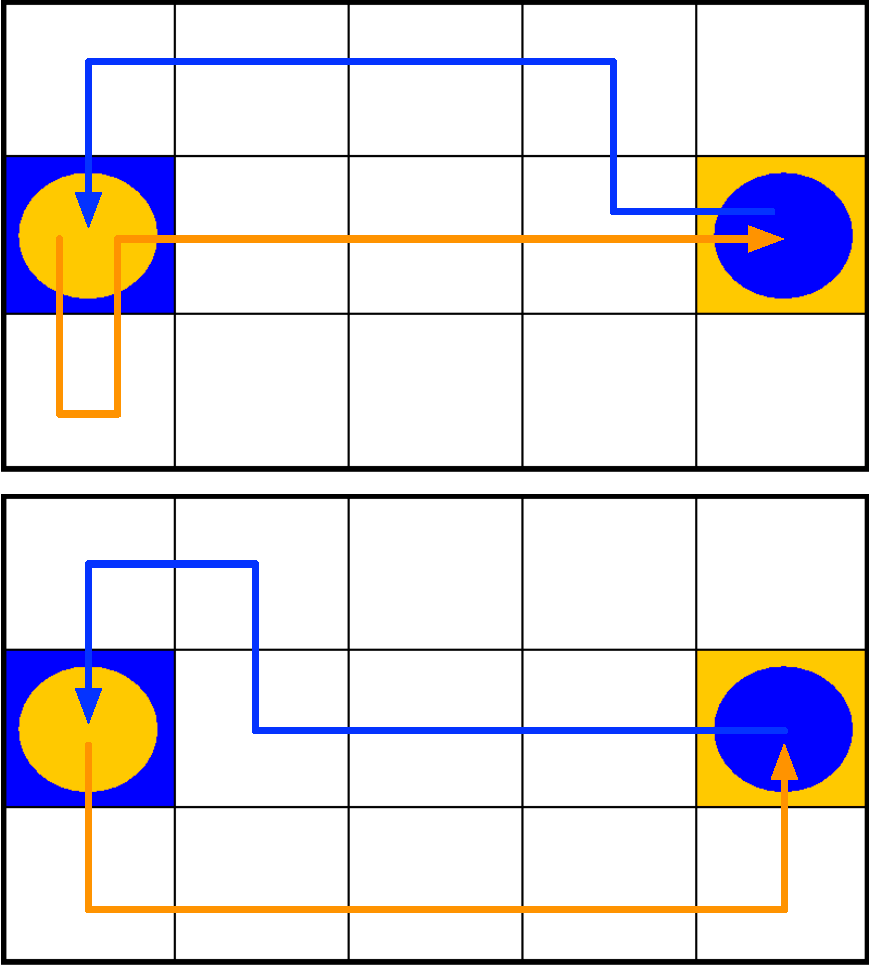
\includegraphics[width=\textwidth]{figures/interactive2}
        \caption{}
        \label{fig:inter2}
    \end{subfigure}
    ~ %add desired spacing between images, e. g. ~, \quad, \qquad, \hfill etc. 
    %(or a blank line to force the subfigure onto a new line)
    \begin{subfigure}[b]{0.18\textwidth}
        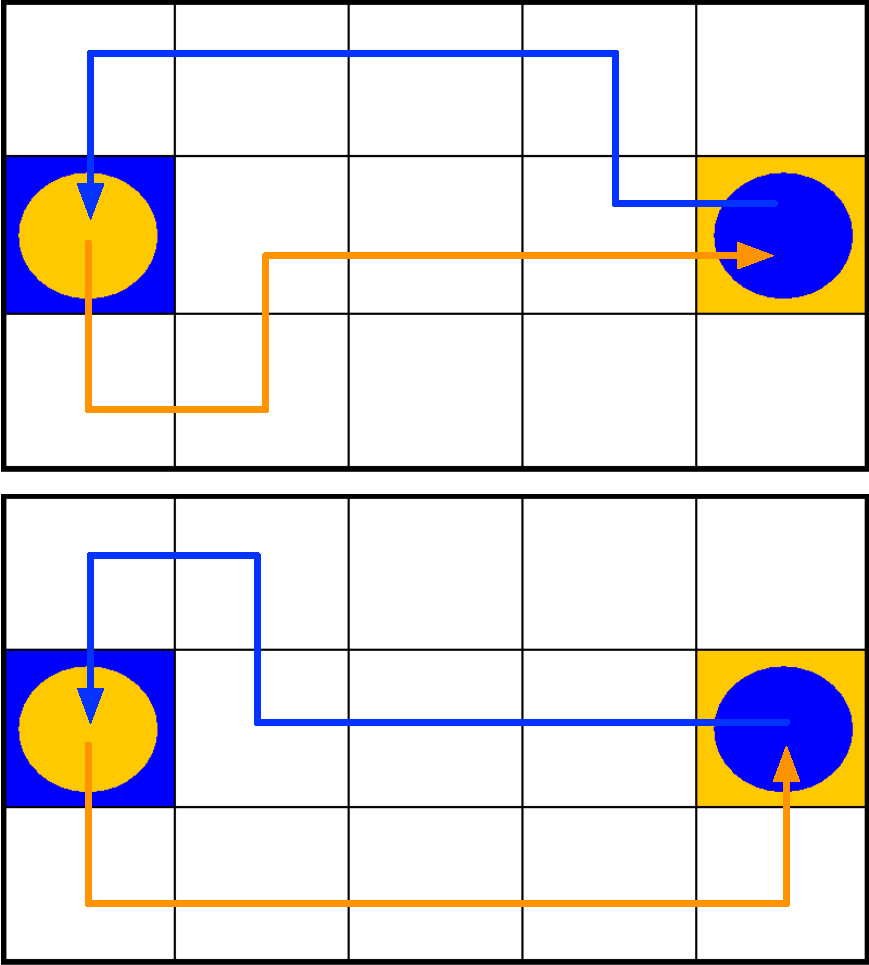
\includegraphics[width=\textwidth]{figures/interactive3}
        \caption{}
        \label{fig:inter3}
    \end{subfigure}
	~ %add desired spacing between images, e. g. ~, \quad, \qquad, \hfill etc. 
    %(or a blank line to force the subfigure onto a new line)
    \begin{subfigure}[b]{0.18\textwidth}
        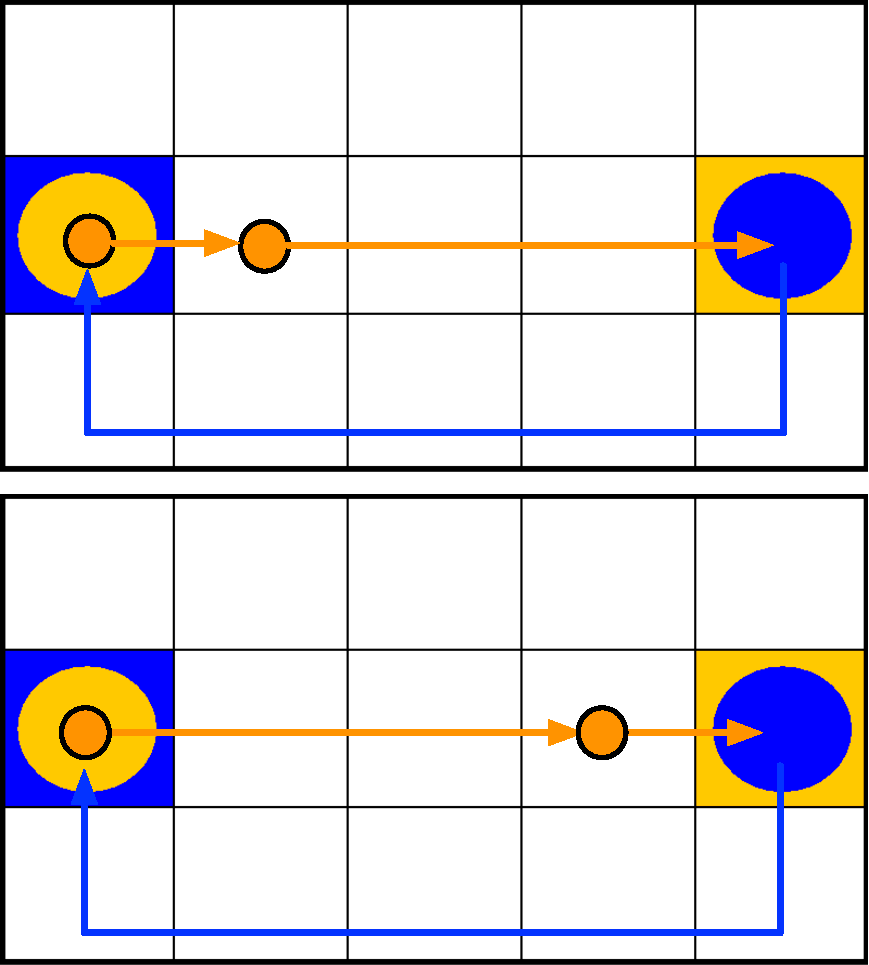
\includegraphics[width=\textwidth]{figures/interactive4}
        \caption{}
        \label{fig:inter4}
    \end{subfigure}
    ~ %add desired spacing between images, e. g. ~, \quad, \qquad, \hfill etc. 
    %(or a blank line to force the subfigure onto a new line)
    \begin{subfigure}[b]{0.18\textwidth}
        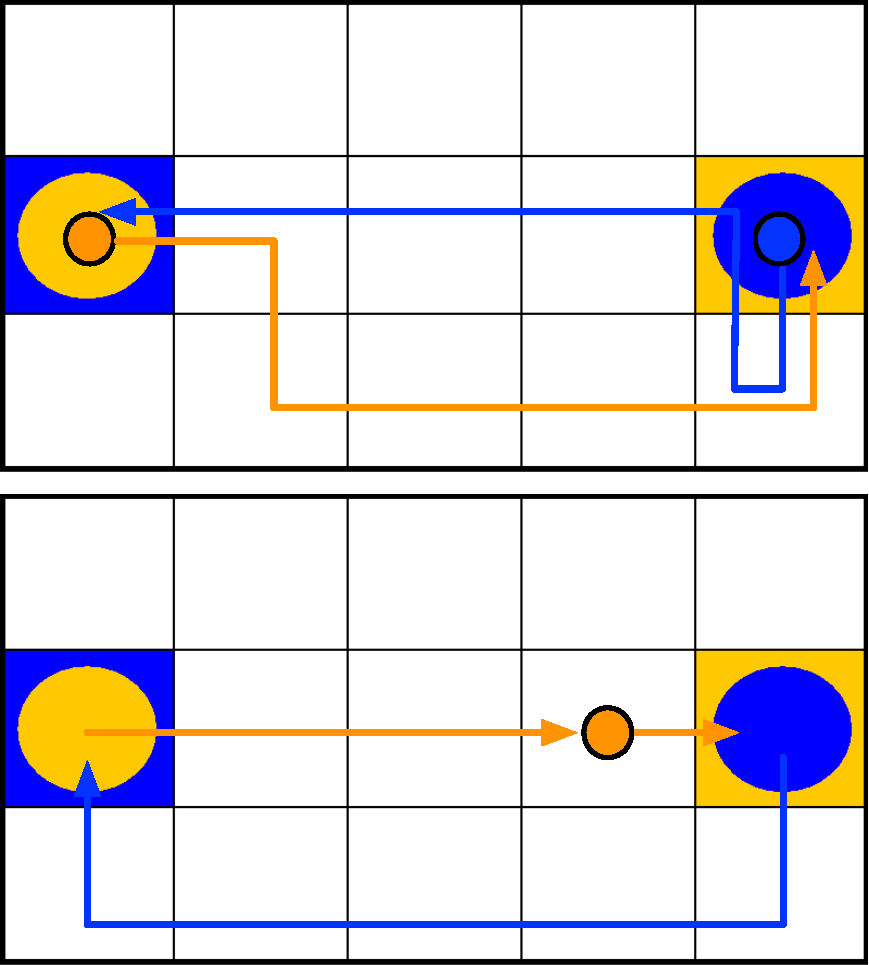
\includegraphics[width=\textwidth]{figures/interactive5}
        \caption{}
        \label{fig:inter5}
    \end{subfigure}
    \caption{The learning results from each of the 5 interactive matches (a-e). The top image for a match is the first round of interaction of the agents. The bottom image for a match is the learned behavior. For matches b-e, the last move of an agent that reaches their goal sooner may be to wait for two steps, or to move north and/or south and back again; only one example is illustrated.}\label{fig:interRes}
\end{figure}

In our interactive norm learning experiment,
%(see Figure~\ref{fig:interRes}), 
we played two interactive learning agents against one another.  The
agents played five matches, each one consisting of five rounds.  Each
match began fresh, without any knowledge of previous matches, to see
whether different norms could emerge.  The social reward function was
initialized to the total welfare joint policy.  In each match, the
agents very quickly (typically after the first round) converged on a
norm that persisted for the rest of the match.  However, in each
match, a different norm was learned, showing that agents employing our
algorithm quickly adapt to the particular shared experience they have
with other agents.
%, and then maintain the learned norm.

Figure~\ref{fig:interRes} shows the results of learning in each of the
five matches (with the top image showing the behavior in the first
round and the bottom image showing the learned behavior). While
different normative behavior was learned in different matches, once
learned, the learned behavior was consistently employed in all
subsequent rounds.  Of particular interest are the results in the
fifth match (Figure~\ref{fig:inter5}). In the first round of this
match, both players wait (a suboptimal joint action), and Blue then
moves in an odd looping motion. Nevertheless, a norm based on the
actions that ultimately worked is learned from the experience, and the
agents do better after that.


%\vspace{\up}
\paragraph{Batch Norm Learning on Human Data}
\label{sec:norm_learning_human}

\begin{table}
\begin{subtable}[t]{0.49\textwidth}
\begin{center}
{\small
\begin{tabular}{|c|c|c|}
\hline
~			& Human vs Human	& Batch Norm IRL	\\ \hline  
Trust			& 76\%			& 72\%			\\ \hline
CD			& 16\%			& 4\%			\\ \hline
Stalemate		& 0\%			& 24\%			\\ \hline
Surrender		& 8\%			& 0\%			\\ \hline
\end{tabular}}
\caption{The percentage classifications of game outcomes for the Amazon Turk experiments and the batch norm learning algorithm trained on the Turk experimental data. The total number of games was $25$.}
\label{tab:batch_human}
\end{center}
\end{subtable}
%
\hfill
\begin{subtable}[t]{0.49\textwidth}
\begin{center}
{\small
\begin{tabular}{|c|c|c|c|c|}
\hline
~			& Trust	& CD	& Stalemate	& Surrender 	\\ \hline
Trust			& 60\%	& 0\%	& 16\%		& 0\%		\\ \hline
CD			& 8\%	& 4\%	& 4\%		& 0\%		\\ \hline
Stalemate		& 0\%	& 0\%	& 0\%		& 0\%		\\ \hline
Surrender		& 4\%	& 0\%	& 4\%		& 0\%		\\ \hline
\end{tabular}}
\caption{The confusion matrix showing how games were classified in the human experiments (row) vs.\ the batch norm learning experiments (column).}
\label{tab:confusion}
\end{center}
\end{subtable}
\end{table}

Finally, we trained our batch norm learning algorithm using data
collected in our 
%human vs.\ human 
Amazon Turk team treatment experiments. The final $10$ trajectories of
each pair of human players was used to train a batch learner that made
decisions for both agents jointly. Table~\ref{tab:batch_human} shows
the classifications of the strategies learned in the $25$ games, while
Table~\ref{tab:confusion} illustrates the learner's ability to create
joint strategies that are classified in the same way as the human
strategies.
%
Like the humans, we can see that the algorithm learned to be trusting
in many cases, and to cooperate defensively in a few.  But the learner
was sometimes unsuccessful at learning a strategy that led either
agent to the goal (even when the humans had managed to reach the
goals), resulting in a fair number of games ending in Stalemate.
%Since the algorithm was making decisions in joint policy space, no surrender strategies were learned.  
Overall, $64\%$ of the policies learned exactly matched the
classification of the human data that was used in training.
Undoubtedly, feature selection plays a major role here,
%Different features would lead to learned strategies that match the training data more or less consistently,
and will be the subject of future research.

%\begin{table}
%\begin{tabular}{|c|c|}
%\hline
%~							& Human $\rightarrow$ Batch Norm IRL	\\ \hline  
%Trust $\rightarrow$ Trust			& 60\%							\\ \hline
%CD $\rightarrow$ CD				& 4\%							\\ \hline
%CD $\rightarrow$ Trust			& 8\%							\\ \hline
%Surrender $\rightarrow$ Trust		& 4\%							\\ \hline
%Surrender $\rightarrow$ Stalemate	& 4\%							\\ \hline
%Trust $\rightarrow$ Stalemate		& 16\%							\\ \hline
%CD $\rightarrow$ Stalemate		& 4\%							\\ \hline
%\end{tabular}
%\caption{This table shows the percentage of games which were classified in a particular way in the human experiments and in the batch norm learning experiments. $A\rightarrow B$ denotes a classification of $A$ in the human case and $B$ for the learner.}
%\label{tab:transfer}
%\end{table}

\comment{
%%% REQUIRES FURTHER DISCUSSION
We see that $64\%$ of the policies learned exactly matched the
classification of the human data that was used in training.  However,
since Surrender and Stalemate policies, and Trust and CD policies,
both lead to the same reward for the agents, the learning algorithm
had a hard time distinguishing between these two pairs of strategies.
}

%In sum, the batch norm learner was not always able to learn a policy that successfully led the agents to their goals.


% 1 page

\section{Plan and Evaluation}
The three year timeline for our proposed project is as follows:

\begin{itemize}
\item {\bf Year 1}: Complete the development of an experimental
  testbed that pairs humans with a (single) artificial agent.
  Demonstrate that the agent can successfully learn norms from batches
  of demonstrations (offline), as well as online, while simultaneously
  interacting with a human.

\item {\bf Year 2}: Investigate methods for greater generalization
  during learning, including methods to generalize norms between state
  spaces and learning norms within {\em populations\/} of interacting
  agents instead of just pairs of agents.

\item {\bf Year 3}: Extend and evaluate our approach in real-world
  applications such as robotic-human collaborations, and develop any
  additional methods necessary to handle these scenarios.
\end{itemize}

In year one, we will develop evaluation metrics, beginning with
experiments evaluating the interactive learning algorithm by comparing
how often and how quickly humans are able to arrive at a social norm
when playing with another artificial agent vs.\ another human.  For
the batch learning component, we will develop new quantitative metrics
to assess trajectory similarity.

We will also develop ways for people to also assess how natural it is
to interact with our artificial agents. For example, we could have two
humans interact for awhile, and then, without notifying them, swap
their partner with an artificial agent trained from the interaction
history. Participants could then be asked if they noticed any change,
and behavior would be compared between cases three cases: no swap,
swapping in a trained agent, and swapping in an untrained agent.

In year two, we will investigate how to transfer and generalize norms
across environments. To facilitate generalization between state
spaces, we will start by examining standard features and
representations used in existing reinforcement-learning 
%RL
and IRL research (e.g., linear models, neural networks, etc.) and
build from them, as necessary, approaches to better capture norms. We
will evaluate generalization by first having users learn a norm in one
grid. Afterwards, they will transfer to a new grid where a ``literal''
norm cannot be directly applied (e.g., adding a wall in the path that
one agent would normally take), but a more ``general'' norm can be
transfered (e.g., I move above the other agent). We will evaluate
these methods using the methods developed in year one.

The algorithms described in this proposal are designed for learning
among a set of agents all playing in same (one) game. We will extend
our work to scenarios where agents play different games, with
different subsets of agents drawn from the same population. We expect
that a group of people can converge on a norm in a setting like this,
and so will extend our algorithms as necessary to support this robust
form of norm-learning. To evaluate our extensions, we will compare
norm formation in purely human groups to hybrid human-machine groups.
%One possible direction is to have the agent learn multiple norms using reward function clustering similar to that in multiple intention IRL\cite{babes11}, and then homogenize the clusters as the populations converges. 
%To evaluate adaptivity in populations, we will compare the results of purely human populations with human-agent populations.

In year three we will test our approach in a real-world domain:
robot-human collaboration. Our simulated worlds suggest that our norm
learning agents could collaborate better with people than traditional
approaches, but the capabilities of robots may inhibit the
effectiveness of our approach (e.g., robots might move slower than
people expect). We will evaluate our algorithm in real-world scenarios
by comparing its performance at controlling a robot to when another
human controls the robot via teleoperation. We expect this to inspire
novel problems tuned to real-world problems. For example, computation
time may be a limiting factor to the success of our machine agents,
and if so, we will develop more efficient implementations.



\section{Deliverables}

The proposed project includes the following deliverables: 

\begin{enumerate}

%%%what does this mean???
%{\em Systematic experimental paradigms\/} 
\item An {\em experimental platform\/} in which humans can interact
  with artificial agents, and that thereby provides a space for
  artificial agents to demonstrate their capacity to represent, learn,
  and ultimately activate norms in context-appropriate ways.

\item {\em Software infrastructure for learning together with
  machine-learning algorithms\/} that enable the representation,
  learning, and activation of norms in simulated stochastic games.
  Code will be made available as a part of the Brown-UMBC
  Reinforcement Learning and Planning
  library\footnote{http://burlap.cs.brown.edu}.

\item Data comprised of the behaviors produced by both humans and
  machines in stochastic games, under varying conditions of complexity
  and uncertainty, as well empirical evaluations of those behaviors.
  These data will form a set of {\em computational benchmarks}, which
  other researchers can freely use to evaluate their own computational
  models of norms.

\item All of the above for coordination problems, specifically.  This
  will produce a set of {\em coordination benchmark}, which we hope
  will inspire other researchers to explore alternative approaches to
  human-machine collaboration.

\end{enumerate}

In year two, we will organize a workshop on the machine learning of
social norms. Such a gathering is timely, as a number of subareas are
grappling with related problems. We will include researchers in
human-robot collaboration~\cite{gopalan15}, intelligent software,
end-user programming of household devices~\cite{ur14}, agent-based
bidding~\cite{tac:book}, multi-agent reinforcement
learning~\cite{sodomka13}, computational social
cognition~\cite{baker14}, and others.

%\subsection{Project Goals}
\label{sec:goals}

This project has three specific goals:

\begin{enumerate}

%\item To use novel human experiments to accumulate and formalize the
%  properties and underlying processes of the human norm system---in
%  particular, the representation and activation of norms.

\item Developing computational formalisms required for representing
  social norms in artificial agents.

\item Showing that norms are learnable by artificial agents in our
  computational representation by developing and evaluating algorithms
  for norm learning in multi-agent settings.

\item Demonstrating a proof of concept by applying our norm
  representation and machine learning algorithms to collaborative
  tasks that involve both humans and machines.

\end{enumerate}



%
\section{Evaluation}
We will evaluate our approach in multiple ways. First, we will test our interactive learning algorithm with other human players in our experimental testbed and compare how often and quickly humans are able to arrive at coordinated plan with our artificial agent versus other humans. To test the expressiveness of our algorithms space of learnable solutions, we will also evaluate how many different kinds of strategies can be found when players play with our agent and compare that to the set of strategies that can be found by humans playing with each other.
Subjective evaluations from the human participants will be used to assess whether interacting with the agent feels natural. 

For the batch learning algorithm, we will develop new quantitative metrics to assess behavior similarity so that trajectories produced from the batch learning can be quantitatively compared to the actual human participants. Additionally, using our experimental test bed, we will have two humans interact for a number of sessions and then, without notification to the users, swap out their partner with an artificial agent trained from the history of interactions they had with their human partner. At the end of all interactions, we will ask the user whether they thought they were playing with the same partner the whole time or if their partner switched. Their subjective response to whether they thought their partner was switched at any point will be compared to their subjective response when their partner is swapped out with an artificial agent that did not perform any learning and when their partner is swapped with a different human player.

Finally, we are also interested in norms generalizing to new state spaces. Using our environmental testbed, we will have participants play in a sequence of different grids and using the same kinds of evaluations listed above, test whether our algorithm can safely generalize to new grids as well as other humans can.

% 1 page

\section{Broader Impacts}

The many devices in our world that collect and share data among the
ever-growing ``Internet of Things" cannot yet intelligently coordinate
their actions to carry out complex tasks without extensive human
programming and configuration.  As this collection of devices grows
and begins to include more traditional robotic actors and more
sophisticated software agents, the need for these entities to not just
communicate but work collaboratively is only going to increase.  We
will want and need them to work together with and without us to
accomplish everyday tasks and help us make better decisions.

The domains that would be positively impacted by machines
that can collaborate effectively with humans is endless, such as robotic sous chefs and
gerontechnological support for aging in place.
%
In particular, the results of this project synergize with the main efforts of 
Brown University's Humanity Centered Robotics Initiative (HCRI), of
which co-PI Littman is co-director. Specifically, within HCRI there
are ongoing efforts to design robotic systems that support independent
living tasks. For an elderly person to trust and collaborate on tasks with a machine effectively, the machine must act in a manner that the elderly person expects. This project lies the foundation for these important applications.

In an effort to increase diversity in computer science, we have
pre-selected two graduate students to participate in this
project---one woman, and the other Hispanic.  All students (both
graduate and undergraduate) who join our team will benefit from collaborating with the cognitive psychologists on our team.
Specifically, they will strengthen their understanding of a number of
fields, all of which are critical to the development of artificial
agents that collaborate effectively with humans: e.g., behavioral
economics, cognitive psychology, reinforcement learning, and software
engineering.

``One of the things that [President Obama] really strongly believe[s]
in is that we need to have more girls interested in math, science, and
engineering.''  To that end, we also plan to integrate our work on
this project into Artemis, a free summer program run at Brown and
directed by PI Greenwald that introduces rising 9th grade girls to
computational thinking.
%\commentj{Explicit mention that this is a STEM priority?}  
For example, we might have the Artemis girls teach a robot to
collaborate with them on various tasks, such as finding and navigating
to common household objects.
%folding laundry.
%\commenta{insert a different example!!!}
%\commenta{You know, girls should be doing housework.} 
% JLA: yeah, i was concerned about the folding laundry example for that reason... 

Our deliverables include an open-source publicly accessible toolkit for machine norm learning via reinforcement learning. Further, we will build a database of machine-machine, human-machine, and human-human experimental results on norm-learning problems, which can serve as a benchmark for future researchers to build artifical agents that increasingly achieve human-like behavior. 
%
Finally, we expect to publish the results of the proposed research in
top-tier archival, conference proceedings and journals with high
impact factors, and present our work at both computer science and
psychology conferences.






\section{Results from Prior NSF Support}

\paragraph{Intellectual Merit}

Greenwald is currently funded by NSF (RI: Small--1217761, 2012--2016,
\$450k) to build artificial agents that assist humans with decision
making in information-rich and time-critical environments like online
markets.  This work is ongoing, but some preliminary publications
include~\cite{tada:jack,seqauc:nips,efgs:rldm,tada:quibids}.
%
Previously, she was funded to develop ``Methods of Empirical Mechanism
Design (EMD)'' (CCF: Medium--0905234, 2009--2012, \$850k, with Mike
Wellman).  This project expanded the scope of mechanism design beyond
the small-scale, stylized, or idealized domains most previous work was
limited to.  Publications include~\cite{poi:aamas,poi:ec,simspsb:uai}.
%
Before that, she received two prior NSF awards, a PECASE CAREER grant,
``Computational Social Choice Theory'' (IIS: Career--0133689,
2002--2007, \$375k), and
%a second award, 
``Efficient Link Analysis'' (IIS: Small--0534586, 2005--2008,
\$363k), which focused on ranking web pages and other social networks
with hierarchical structure.

\comment{
(iii)	Results from Prior NSF Support

If any PI or co-PI identified on the project has received NSF funding in the past five years, information on the award(s) is required. Each PI and co-PI who has received more than one award(excluding amendments) must report on the award most closely related to the proposal. The following information must be provided:

(a)	the NSF award number, amount and period of support;

(b)	the title of the project;

(c)	a summary of the results of the completed work, including, for a research project, any contribution to the development of human resources in science and engineering;

(d)	publications resulting from the NSF award;

(e)	a brief description of available data, samples, physical collections and other related research products not described elsewhere; and

(f)	if the proposal is for renewed support, a description of the relation of the completed work to the proposed work.

Reviewers will be asked to comment on the quality of the prior work described in this section of the proposal. Please note that the proposal may contain up to five pages to describe the results. Results may be summarized in fewer than five pages, which would give the balance of the 15 pages for the Project Description.
}

Littman is a co-PI on ``RI: Medium: Collaborative Research: Teaching
Computers to Follow Verbal Instructions'' (No.\ 1065195, 9/11--8/14,
\$704K) and ``RI: Small: Collaborative Research: Speeding Up Learning
through Modeling the Pragmatics of Training'' (No.\ 1319305,
10/13--9/15, \$440k). These proposals developed autonomous agents that
extract preferences from people via verbal interaction and reward
feedback~\cite{loftin14b,macglashan15,macglashan15b}.

\paragraph{Broader Impact}

Broader impacts of our past work include undergraduate and graduate
student training, design and evaluation of learning modules for
outreach programs Learning Exchange and Artemis, and organizing two
major computer science conferences (Littman)~\cite{desjardins13}.
We also published novel benchmarks for evaluating grounded language
learning programs (Littman), and developed a simulation platform for
empirical game-theoretic analysis (Greenwald).

Greenwald also had an additional NSF award (EAGER: 1059570,
2010--2012, \$90k) which supported the expansion and evaluation of the
Artemis Project, a free, summer program in which Brown computer
science women teach computer science to rising 9th grade girls.  This
program has the dual effect of empowering Brown women, while at the
same time, exposing girls to computer science.  With this money, she
successfully expanded Artemis to BU, and ran pilot programs at
Columbia and UMBC.

Greenwald also has \$10k in funding from the Tides Foundation, through
the IgniteCS progam, for a project entitled Bringing Computer Science
Education to Providence Public Schools.



\newpage
\setlength{\itemsep}{0pt}
\setcounter{page}{1}

\bibliographystyle{plain}
\bibliography{grant}

\end{document}

